\documentclass[preprint,10pt,numbers]{elsarticle}

% amsmath package, useful for mathematical formulas
\usepackage{amsmath}
% amssymb package, useful for mathematical symbols
\usepackage{amssymb}

% graphicx package, useful for including eps and pdf graphics
% include graphics with the command \includegraphics
\usepackage{graphicx}

% cite package, to clean up citations in the main text. Do not remove.
%\usepackage{cite}
\usepackage[]{natbib}

\usepackage{color} 

% Use doublespacing - comment out for single spacing
\usepackage{setspace} 
\doublespacing

\usepackage{xr}
\externaldocument{chemokine_supplement_revised}


% Text layout
\topmargin 0.0cm
\oddsidemargin 0.5cm
\evensidemargin 0.5cm
\textwidth 16cm 
\textheight 21cm

% Bold the 'Figure #' in the caption and separate it with a period
% Captions will be left justified
\usepackage[labelfont=bf,labelsep=period,justification=raggedright]{caption}

%\bibliographystyle{elsarticle-num}
\bibliographystyle{elsarticle-num-names}
%\bibliographystyle{plos2009}

% Remove brackets from numbering in List of References
\makeatletter
\renewcommand{\@biblabel}[1]{\quad#1.}
\makeatother


% Leave date blank
\date{}

\pagestyle{myheadings}
%% ** EDIT HERE **


%% ** EDIT HERE **
%% PLEASE INCLUDE ALL MACROS BELOW

\usepackage{multirow}
\renewcommand{\arraystretch}{1.1}

% figure files reside in the figures/ directory
\graphicspath{
{figures/}
}

\usepackage{color}
\usepackage[usenames,dvipsnames,table]{xcolor}
\usepackage{ulem}

%\usepackage[normalem]{ulem}

\definecolor{dkred}{rgb}{0.75,0,0}
\definecolor{dkgreen}{rgb}{0,0.5,0}
\definecolor{dkblue}{rgb}{0,0,0.75}
\definecolor{dkpurple}{rgb}{.375,0,.375}
\definecolor{gray}{rgb}{0.5,0.5,0.5}

%\newcommand{\removed}[1]{{\color{dkred}\sout{#1}}}
%\newcommand{\new}[1]{{\color{dkgreen}#1}}
\newcommand{\removed}[1]{}
\newcommand{\new}[1]{#1}
\newcommand{\drew}[1]{{\color{dkgreen}#1}}
\newcommand{\fred}[1]{{\color{dkblue}#1}}
\newcommand{\steph}[1]{{\color{dkpurple}#1}}

\journal{Theoretical Biology}

%% END MACROS SECTION

\begin{document}

% Title must be 150 characters or less
\begin{flushleft}
{\Large
\textbf{A spatial model of the efficiency of T cell search in the influenza-infected lung}
}
% Insert Author names, affiliations and corresponding author email.
\\
Drew Levin$^{1,\ast}$, 
Stephanie Forrest$^{1}$, 
Soumya Banerjee$^{1}$,
Candice Clay$^{2}$, 
Judy Cannon$^{3}$,
Melanie Moses$^{1}$, 
Frederick Koster$^{1,2}$
\\
\bf{1} Department of Computer Science, University of New Mexico, Albuquerque, NM, USA
\\
\bf{2} Lovelace Respiratory Research Institute, Albuquerque, NM, USA
\\
\bf{3} Department of Molecular Genetics \& Microbiology Department of Pathology, University of New Mexico Health Sciences Center, Albuquerque, NM, USA
\\
$\ast$ E-mail: Corresponding drew@cs.unm.edu
\end{flushleft}



% Please keep the abstract between 250 and 300 words
\section*{Abstract}

%Emerging strains of influenza, such as avian H5N1 and 2009 pandemic H1N1, are more virulent than seasonal H1N1 influenza, yet the underlying mechanisms for these differences are not well understood.  Viral clearance depends in part on the ability of T cells to locate the infection in time to prevent uncontrolled spread of the virus.  We use an agent-based spatial model to quantify how efficiently T cells locate and control different strains of influenza in the lung.  We calibrate the model using viral and chemokine secretion rates measured \textit{in vitro} for avian H5N1, seasonal H1N1, and 2009 pandemic H1N1 influenza, together with values taken from literature.  The spatial model reveals challenges for T cell recruitment not apparent in standard differential equation models.  The model shows that virus kinetics largely determine the course of the infection, especially in the case of the pandemic flu strain, while T cell control of the seasonal flu strain is more important. Our results shed light on the key factors differentiating immune response against seasonal, avian, and pandemic flu.

%while T cell chemokine parameters have less effect.

%Further analysis of the model identifies the viral parameters as most significant and suggests possible mitigation strategies.

% ---- 300-ish word abstract

Emerging strains of influenza, such as avian H5N1 and 2009 pandemic H1N1, are more virulent than seasonal H1N1 influenza, yet the underlying mechanisms for these differences are not well understood.  Subtle differences in how a given strain interacts with the immune system are likely a key factor in determining virulence.  One aspect of the interaction is the ability of T cells to locate the foci of the infection in time to prevent uncontrolled expansion.  Here, we develop an agent based spatial model to focus on T cell migration from lymph nodes through the vascular system to sites of infection. We use our model to investigate whether different strains of influenza modulate this process.

We calibrate the model using viral and chemokine secretion rates we measure \textit{in vitro} together with values taken from literature.  The spatial nature of the model reveals unique challenges for T cell recruitment that are not apparent in standard differential equation models.  % -- Fred --
%We find that as plaques expand in size, the ratio of infected cells to dead cells decreases, making it difficult for T cells to encounter infected cells efficiently.  Further, differences in the diffusion rates of chemokines and virions can misdirect T cells to areas that no longer contain infected epithelial cells.  While our sensitivity analysis identifies viral parameters as the most significant factor in determining the course of the infection, we are also able to determine an upper bound of T cell search time using the model.  Finally, we use the model parameters to determine an upper bound on T cell search time in the model.  Our results shed light on the key factors differentiating immune response against seasonal, avian, and pandemic flu.
% -- Fred , after p2s2 -- 
In this model comparing three influenza viruses, plaque expansion is governed primarily by the replication rate of the virus strain, and the efficiency of the T cell search-and-kill is limited by the density of infected epithelial cells in each plaque.  Thus for each virus there is a different threshold of T cell search time above which recruited T cells are unable to control further expansion.  Future models could use this relationship to more accurately predict control of the infection.

% ---- end 300-ish word abstract

% To determine local chemokine production, avian H5N1, seasonal H1N1, and 2009 H1N1 pandemic influenza strains were used \textit{in vitro} to induce the secretion of CXCL10 (IP-10) and CCL5 (RANTES) in human bronchial epithelial cells.  These data were fit to a differential equation model in order estimate viral and chemokine production rates. 

% Infected cells can become isolated in expanding plaques, impeding T cell search, even though the T cells could directionally migrate to low levels of chemokine.  This spatially explicit model describes efficient T cell recruitment to small infected foci in the lung, but as foci become large T cell search becomes inefficient, thus emphasizing the importance of enhanced control early in infection.  A key limitation imposed on T cells is illustrated by their failure to clear the pandemic H1N1 virus after day 6, when T cells became inefficient in finding infected cells in large foci.    Thus, we conclude that viral dynamics, rather than chemokine dynamics, dominate the efficiency of T cell recruitment in determining whether the influenza infection is controlled.


\section*{Keywords}

Agent-Based Model, Systems Biology, Immunology, Computational Biology, Virology


\section*{Introduction}

Influenza has worldwide epidemic potential with 5 million infections annually and half a million deaths \citep{Who2009}.  Emerging strains of influenza, such as 2003 H5N1 avian and 2009 H1N1 pandemic, are more pathogenic than seasonal strains, yet the mechanisms that control this variability are not well understood.  Pathogenicity is a function of both the virus and its interaction with the immune response. Our model explores how various features of the virus and the host immune system interact to produce observed differences between strains.

Identifying the critical components of this complex process, and how they interact, is key to understanding viral pathogenicity and designing therapeutic interventions.  We address this challenge through computational modeling, which allows us to study the relative contributions of different aspects of the host immune response and to account for strain-specific viral dynamics in the model.  Several earlier theoretical models have been proposed to study specific aspects of influenza infections. Ordinary differential equation (ODE) models that are fit to empirical data \citep{Handel2008, Lee2009, Miao2010a, Saenz2010, Murillo2013, Crauste2015, Price2015} have elucidated viral population level dynamics but are unable to perceive localized spatial effects.  Spatial models, on the other hand, have been developed to examine interactions between dendritic cells and T cells in the lymph node \citep{Beauchemin2005, Beltman2007, Zheng2008, Mirsky2011, Celli2012, Vroomans2012, Textor2014}, but have not been extended to consider local conditions in the lung.   In this paper, we examine how the unique properties of three different strains of influenza, in the presence of chemokines, affect T-cell search in the human lung.

Specifically, we focus on the interactions between activated antigen-specific CD8 T cells, cytokines, and replicating influenza virus.  Chemotactic proteins are known to enhance T cell recruitment in both acute infections and chronic inflammatory diseases \citep{Gunn1998, Medoff2005, Okada2005, Castellino2006, Bromley2008}. Infected epithelial cells secrete chemokines, especially upon contact with CD8 T cells  \citep{Zhao2000, Chan2005}. Previous work showed that efficient recruitment of T cells to the Focus Of Infection (FOI) is crucial for the eventual clearance of the virus\citep{Cerwenka1999, Kim2011}.   As measuring real-time T cell movement in \textit{in vivo} lung tissue is not currently viable, study these localized processes is aided by spatial modeling of how T cells interact with the FOI and the chemotactic environment.  Therefore, instead of developing a comprehensive immune system model, we present a spatially explicit agent-based model (ABM) to describe T cell interactions with chemotactic signals and a dynamically growing plaque.  Using the model, we investigate the pathogenic potential of the three  influenza strains: seasonal H1N1 (sH1N1), Avian H5N1 (aH5N1), and pandemic H1N1 (pH1N1). These three strains were selected for their differences in \textit{in vitro} replication rates \citep{Mitchell2011} as well as differences in \textit{in vivo} severity of human and animal pneumonia and mortality.

The model is parameterized with values taken from the literature when available.  Because chemokine secretion rates are central to our model and appropriate data values are not available, we estimate the parameters using data from physical experiments and our previously published ODE model \citep{Mitchell2011}.   

To obtain the physical data, wells of human epithelial cells were infected with one of the three strains and then measured for virus and cytokine concentrations over a 48-hour period.   Of the cytokines tested, only the chemokines CXCL10 (IP-10) and CCL5 (RANTES) were expressed differently across the three influenza strains.   IP-10 and RANTES are both chemokines that normally attract T cells to the FOI \citep{Hoji2005, Groom2011a}.  These results suggest that the two chemokines may contribute to the immune system's varying ability to control different strains of influenza, and were thus included in our model.

The analyses of the spatial model reveal several interesting and underappreciated phenomena.  The model identified physical constraints on T cells' ability to clear the rapidly replicating pH1N1 infection. Because T cells in the model use the chemokine gradient to locate the FOI, they tend to cluster in areas of high chemokine concentration. The model suggests that the chemokine response of the host cells can hinder T cells’ ability to find and clear infected cells in the presence of the rapidly replicating pandemic strain. A sensitivity analysis of the model parameters isolated the effects of each parameter in the model.  The analysis shows that most model parameters can vary across a broad range of values without strong effect on predicted outcomes.  Further analysis shows model predictions remain unchanged within broad categories of parameter type (e.g., all parameters related to chemokines, parameters related to viral kinetics, etc.).  For example, the chemokine-related parameters are stable in that they do not affect the model behavior within biologically plausible ranges. In contrast, parameters related to viral kinetics significantly alter model predictions.  Finally we examine the `window of control' which establishes an upper bound on the time it takes T cells to arrive at the FOI while still clearing the infection.  We find that this value is consistent with our sensitivity analysis and helps explain the challenge of controlling the highly virulent pH1N1 strain.



%We conclude that influenza infection dynamics are dominated by the replication properties of the virus and spatial properties of the infection. The higher replication rate of 2009 pH1N1 influenza dominated the effect of chemotactic signals, leading to uncontrolled infection \textit{in silico}.


\section*{Methods and Models}

% We are interested in how the interaction between the virus and the host's secondary immune response affects the virulence of the infection.  Because these interactions are difficult and expensive to observe \textit{in vivo}, we create a model \textit{in silico} to represent the system in question.  Because we are interested in individual interactions between the virus and the immune response, as well as the spatial nature of the spreading infection and the subsequent T cell search, we eschew traditional differential equation models \citep{Beauchemin2006a, Bauer2009} in favor of a spatial agent-based model (ABM).  

% Our modeling methodology follows three steps.  First, we define the system we are going to model.  Second, we build the model with this definition in mind.  Finally, we parameterize the model using empirical data, values from literature, and computational techniques.

\subsection*{Model Definition}

%Our model examines the secondary immune response to an influenza infection in a human lung.  Specifically, we are interested in how antigen activated T cells efficiently navigate from the lymph node, through vascular system, and into the lung at the site of infection.  

The model focuses on activated CD8 T cells migrating through the vascular and lymph networks, including their movement over tissue after extravasation (Fig.~\ref{fig:systemchart}).  While the volume of the lung consists of spherical alveoli, the spread of influenza throughout the lung occurs through the interconnected bronchiole-alveoli complex, which can be viewed as a connected monolayer.  Thus, we represent the lung as a two-dimensional sheet of healthy epithelial cells (S1.3).   Because we assume activated T cells descend at random into branches of the vascular network, T cells in the model are introduced uniformly at random across the modeled lung surface.  If cytokine signal is detected on the local endothelium the T cell remains in tissue and follows the chemotactic gradient to the FOI.  T cells that do not encounter cytokine recirculate to the lymph node where they reenter the bronchial vascular network.  Once inside the endothelium, T cells follow the chemokine gradient to localized areas of maximum chemokine concentration.  When a T cell contacts an infected epithelial cell it induces apoptosis (S1.4).  Otherwise, infected cells continue to secrete virus for a fixed time and then die.

The model is initialized with a single infected cell.  After the incubation period, the infected cell begins secreting virus and chemokine at rates determined by the virus strain and chemokine type (Table \ref{tab:strains}).  Virus from expressing cells diffuses locally, infecting neighboring cells. Chemokine diffuses from secreting cells, creating a spreading region of stimulation around the FOI. After four simulated days, Immunoglobulin M (IgM) is introduced into the model by increasing the viral decay rate.  After five simulated days, representing lymph node stimulation and T cell proliferation, activated T cells exit the lymph node at a constant rate and travel through the vasculature to the tissue as described above.  These cell and molecular interactions and state transitions are depicted in Figure~\ref{fig:systemchart}.

\subsection*{Model Parameters}

We include only parameters that directly address the role of T cells and T cell migration because our study focuses on the role of T cells and the chemokine effects of T cells in influenza virus infection. Thus, we included parameters that affected virus, T cells, and chemokines. With regards to the influenza, we chose parameters involving viral replication, infectivity in epithelial cells, and virus decay and diffusion rates based on our earlier study.  The chemokine decay rate, diffusion rate, and secretion rate parameters are relevant to dynamic chemokine gradients required for T cell chemotaxis.  Because we wanted to use our model to test the role of T cells and T cell migration in influenza clearance, we included multiple T cell parameters, such as T cell production rate, T cell death rate, T cell kill time, and T cell migration rate.  We added IgM because many studies have argued for the importance of antibody mediated virus clearance. However, because our study is not addressing the role of antibody in clearance of influenza, we did not test the full range of B cell responses directly by including them in our parameters.

Model parameters are listed in Tables \ref{tab:strains} and \ref{tab:parameters}. These values were taken from the literature when available.  Other parameters were determined by matching empirical data to ODE models, and some parameters were estimated using biologically plausible ranges.  All estimated parameters were studied in a sensitivity analysis to test their impact on model behavior (Table~\ref{tab:sensitivity}). 

Because we are interested in the interplay between the virus and the induced immune response, we infected human epithelial cells with the three different strains of influenza \textit{in vitro} and measured the resulting cytokine and chemokine responses.  We extended our previously published differential equation model \citep{Mitchell2011} to obtain values for per-cell chemokine production rates.  T cell production rates were derived from measured replication rates \textit{in vitro} \citep{Miao2010a} using another differential equation model. T cell production is assumed to be constant after day 5 \citep{MartIn-Fontecha2003}.  

\subsection*{Model Implementation}

The model is implemented using an updated version of the CyCells software \citep{Warrender2006},
(\texttt{github.com/drewlevin/cycells}),
a modeling platform for two- or three-dimensional agent-based simulations of the immune response (S1.1).  Due to computational constrains our model is scaled to the size of a mouse lung (approximately 100$cm^2$), a well-established practice in spatially explicit influenza models \citep{Miller2003, Allan2006, Ingulli2009}.  Parameters affected by this choice include the T cell production rate, T cell circulation time, and the total size of the lung (Table \ref{tab:parameters}).

Parameters that are independent of the chosen influenza strain are shown in Table \ref{tab:parameters}.  Strain-specific values are shown in Table \ref{tab:strains}.  Further details regarding the model definition are included in S1.2.

In the model, epithelial cells are stationary and are described by one of five sequential states: \texttt{healthy}, \texttt{virus-incubating}, \texttt{virus-expressing}, \texttt{apoptotic}, and \texttt{dead} \citep{bachem1996simulated, Beauchemin2005, Mitchell2011}. \texttt{Healthy} cells remain unchanged unless infected by virus. Once infected, the cell transitions from \texttt{incubating} to \texttt{expressing} after a 10 hour incubation delay (Table \ref{tab:parameters}). \texttt{Expressing} cells secrete virus and chemokine for a fixed 16.7 hours and then die (Table \ref{tab:parameters}). \texttt{Expressing} cells initiate apoptosis sooner if they are contacted by activated T cells. \texttt{Apoptoic} cells continue to secrete virus and chemokine and then die after one hour (Table \ref{tab:parameters}). \texttt{Dead} cells take up space and do not regenerate over the course of an infection.  Cell regrowth is not implemented as the rate of regrowth is unknown. 

T cells are described by two states: \texttt{circulating} and \texttt{chemotaxing}.    T cells emerge from the lymph node at five days post infection (p.i.) at a rate of 1,257 cells per hour (Models for Parameter Estimation, Table \ref{tab:parameters}). T cell travel time from the lymph node to a random location on the lung's surface is six seconds.  If chemokine is not encountered, the circulating T cell returns to a new location in the lung after another six seconds.  If a circulating cell encounters chemokine, it changes state to \texttt{chemotaxing} and follows the chemotactic gradient to the FOI. Circulating T cells decay exponentially with an average lifespan of four days.  Chemotaxing T cells follow the gradient through the two-dimensional lung endothelium, inducing apoptosis when they encounter expressing epithelial cells. Chemotaxing T cells decay exponentially with an average lifespan of two hours.  Justifications for these parameter values are listed in Table \ref{tab:parameters}.

In addition to T cells, the model contains two types of particles: virus and chemokine. Both are produced at constant rates by expressing epithelial cells.  Virus diffuses through the lung tissue, infecting healthy cells at a rate proportional to the virus concentration at the location of the cell. Chemokine diffuses across the tissue but has no direct effect beyond recruiting T cells. Both particle types decay exponentially.  IgM is modeled by increasing the viral decay rate by a factor of ten after the fourth day (Table \ref{tab:parameters}).

\subsection*{Models for Parameter Estimation}

To provide estimates of chemokine concentrations and secretion rates in lung tissue, chemokine levels were measured at 4-6h intervals during the first 48 h of infection in wells containing approximately one million human bronchial epithelial cells (Fig. \ref{fig:data}, Table \ref{tab:data}).  The dynamic viral loads at these intervals have been reported previously by us for cultures infected with seasonal H1N1 virus, pandemic H1N1 virus, and avian H5N1 virus \citep{Mitchell2011}.  IP-10 concentration increases were observed by 8h post-infection (p.i.), and RANTES by 16h p.i..

We estimate chemokine production rates, $r$, by adapting the delay differential equation model of influenza infection described in \citep{Mitchell2011} Eq. 1 by adding one new equation ($\dot{C}=r I_{1 \tau_3}-dC$) to model chemokine production.   Strain-specific values for $r$ were found by fitting the equations to the experimental data in Table~\ref{tab:data} using a genetic algorithm to minimize the log squared error between the model and the data while holding the rest of the parameter values constant \new{(Fig. S1, Table~\ref{tab:rmse})}.  Next, 1,000 bootstrapping runs using resampled residuals were performed on each modeled strain to generate confidence intervals over $r$.  The results of these fits are shown in Table 1 (viral secretion rates are from previous fits in \cite{Mitchell2011}).  IP-10 and RANTES secretion rates are aggregated in the spatial model (S2.2).

{\footnotesize
\begin{equation*}
\begin{aligned}
\dot{T} &= - \beta T V \\
\dot{I_1} &= \beta T V - \beta T_{\tau_1}V_{\tau_1} \\
\dot{I_2} &= \beta T_{\tau_1}V_{\tau_1} - \delta I_2 \\
\dot{V} &= \frac{p}{1+eF} I_2  - \beta T V  \\
\dot{F} &=  I_{1 \tau_2} \\
\dot{C} &= r I_{1 \tau_3} - d C \\
\end{aligned}
\tag{Eq. 1}
\label{eq:dde}
\end{equation*}
\vspace{.05in}
}
$\tau$ subscript variables denote delay terms, signifying the value is the population quantity in existence at time $t - \tau$.  Table \ref{tab:dde} summarizes population and parameter values and descriptions.  

%\subsection*{Chemokine Secretion}


% Model fits (Table \ref{tab:strains}) were computed for three strains using Matlab's \texttt{nlinfit} function (Levenberg-Marquardt algorithm).  The resulting chemokine production values were used in the CyCells ABM by combining IP-10 and RANTES into one aggregate rate but also reported separately (Fig.~S2).  Best-fit expression rates were similar for all strains except for significantly higher RANTES production in aH5N1.  There was no positive correlation between viral production and induced chemokine production across the three strains.


% \subsection{Estimating the T cell production rate}

We calculate the rate of production, $\sigma$, of CD8 T cells using a differential equation model from \citep{Miao2010a}.  The equations model T cell production and subsequent search over an area of infected lung tissue.

{\footnotesize
\begin{equation*}
\label{eq:miao}
\begin{aligned}
\dot{N_{c}} &= \sigma - \frac{r'^{2} \cdot N_{c}}{R^{2} \cdot t_{rc}} & \pi r'^{2} &= a \sqrt{I} + b \\
\dot{N'_{f}} &= \frac{(r'^{2} - r^{2}) \cdot N_{c}}{R^{2} \cdot t_{rc}} - \frac{v_{tcell}}{(r' - r) / 2} \hspace*{2cm}  & \pi r^{2} &= \pi r_{cell}^{2} \cdot I \\
\dot{N_{f}} &= \frac{r^{2} \cdot N_{c}}{R^{2} \cdot t_{rc}} + \frac{v_{tcell}}{(r' - r) / 2} \\
\dot{T} &= \rho T -\beta TV \\
\dot{I} &= \beta TV - \delta I - k_{e} N_{f} I \\
\dot{V} &= pI - \beta TV - \gamma (t) V \\
\gamma (t) &= \left\{ \begin{array}{rcl}
	1/\mbox{day} & \mbox{,}  & t < 5  \\
	3/\mbox{day} & \mbox{,} & t \geq 5  
	\end{array}\right. \\
\end{aligned}
\tag{Eq. 2}
\end{equation*}
}
\vspace{0.5in}


$N_{c}$ is the number of circulating activated antigen-specific CD8 T cells, $N'_{f}$ is the number of circulating T cells that have found and exit into a region of lung tissue expressing chemokines, $N_{f}$ is the number of circulating T cells that have found an infected region. $T$ is the number of uninfected target cells, $I$ is the number of productively infected cells, and $V$ is the viral titer in serum. The infected region is assumed to be of radius $r$ and is within a region expressing chemokines of radius $r'$ ($r  < r'$). The lung is modeled as a circular region with radius $R$. The area of the infected region is equal to the area of an infected cell (of radius $r_{cell}$) multiplied by the number of infected cells. See Fig.\ref{fig:systemchart} for more details about the model.  The area of the region expressing chemokine was found to be related non-linearly to the number of infected cells ($\pi r'^{2} = a \sqrt{I} + b$) where $a$ and $b$ are constants that depend on the viral strain.  $a$ and $b$ were fit to 5 experimental runs of a spatial model implemented in CyCells ($R^2 = 0.997$, $P < 0.01$).

Circulating CD8 T cells ($N_{c}$) are assumed to be released from lymph nodes at a constant rate $\sigma$ and circulate to the $N'_{f}$ population over a time defined by $t_{rc}$. We assume these circulating cells transition into $N'_{f}$ and $N_{f}$ at rates proportional to the areas of the chemokine expressing and infected regions relative to the whole lung area. 

The average time an exiting CD8 T cell takes to migrate to the infected region is equal to the difference in the radii between the two regions ($r' - r$) times the T cell speed, $v_{tcell}$.  Circulating cells that are in the chemokine expressing region ($N'_{f}$) move into the infected region after performing chemotaxis for that time. Target cells ($T$) become infected by virus at rate $\beta TV$, where $\beta$ is the rate constant characterizing infection. Infected cells ($I$) die at rate $\delta$ in addition to being lysed by T cells ($N_{f}$) at a rate $k_{e}$. Finally the viral titers ($V$) increase due to production of virus at rate $p$ by infected cells. Virus is also cleared due to uptake by infected cells (at a rate $- \beta TV$) and due to antibody (at a rate $\gamma (t)$ that changes after 5 days post infection). The initial viral titer was initialized to 10,000 PFUs and the initial number of target cells was one million. The initial number of infected cells is assumed to be zero. Parameter values are listed in Table \ref{tab:supplement}.  This ODE was fit to data taken from \citep{Miao2010a} using Matlab's \texttt{nlinfit} function in order to obtain a value for $\sigma$.  The final value was found to be 1,257 per hour.


\subsection*{Materials}

In an effort to obtain per-cell chemokine and cytokine production rates, human epithelial cells were infected with influenza \textit{in vitro}.  Epithelial cell culture and supernatant collection was performed as described in \citep{Mitchell2011}.  Briefly, undifferentiated human tracheal epithelial cells (University of Miami) were cultured for 4 weeks to achieve fully differentiated confluent monolayers on collagen-coated transwell inserts, or commercial differentiated human bronchial epithelial cells (EpiAirway Tissue, MatTek Corp., Ashland, MA) used immediately upon receipt, were infected at an MOI of 0.01 with either seasonal H1N1 virus A/New Caledonia/20/99 (sH1N1), the 2009 H1N1 pandemic strain A/California/04/09 (pH1N1), or avian H5N1 virus A/Hong Kong/483/97 (aH5N1) derived from a fatal human infection.  Basal media was collected from previously undisturbed triplicate or quadruplicate wells at 0, 6, 10, 12, 16, 20, 24, 30, 36, 42, 48, and 72 hours after infection, and stored at -80C until assay.  Subsequently, apical fluid for virus secretion was collected before and after treatment of the monolayer with protease (Pronase, Sigma) to optimize the collection of infectious virus \citep{Mitchell2011}.  Quantitative viral culture was performed by standard plaque assay.  Quantitative chemokine levels were performed in 30 $\mu$L aliquots for a panel of chemokines (IL-8, MCP-1, MIP-1$\alpha$, MIP-1$\beta$, RANTES, IP-10, eotaxin) and cytokines (interferon-gamma, IL-1$\alpha$, IL-1$\beta$, IL-1RA, IL-2, IL-3, IL-4, IL-6, IL-10, IL-12p40, IL-15, IL-17, TNF$\alpha$) (Luminex Assay®, Luminex Corp.) and reported as ng/mL basal media sampled from a total volume of 4 mL.  Only IP-10, RANTES, and TNF$\alpha$ showed increases in production (Table \ref{tab:data}).  TNF activity is not incorporated in the model.  Data for other chemokines and cytokines is not shown.



\section*{Results}

\subsection*{Model Results}

Because the CyCells model is stochastic, we conducted 100 runs of the model with the same parameter set for each of the three influenza strains, each run initialized with a unique random seed (Fig.~\ref{fig:variance}).  We count the number of infected cells in the simulated plaque at every time point.  For the avian and seasonal strains, all model runs cleared the infection by day 10.  Conversely, each simulation of the 2009 pandemic influenza led to uncontrolled infection. 

% We estimated variance across the runs using the $R^2$ statistic, $\pm$ one standard deviation: 0.957 $\pm$ 0.150 (avian), 0.992 $\pm$ 0.013 (seasonal), and 0.998 $\pm$ .002 (pandemic).  The $R^2$ was computed with respect to the mean number of infected cells at each simluated time point across all 50 runs. Consistent with earlier results \citep{Mitchell2011}, the time course of the infection varies significantly across the three strains (Fig.~\ref{fig:variance}).

We estimated variance across runs by calculating the standard deviation at each time point.  For aH5N1, the maximum standard deviation was 35, which occurred at day 4.8 where the mean value was 257.  For sH1N1, the maximum standard deviation was 212, which occurred at day 5.1 where the mean value was 2,528.  For pH1N1, the maximum standard deviation was 231, which occurred at day 5.1 where the mean value was 6,988 (Fig.~\ref{fig:variance}).

In all studied strains, virus population growth slows at four days p.i. (Fig.~\ref{fig:variance}), due to IgM appearance.  Subsequently, the simulated CD8 T cell response causes the number of infected cells to decline quickly after day five p.i.  aH5N1 is cleared completely, sH1N1 is cleared more slowly.  In contrast, at day six p.i., pH1N1 replication overwhelms the IgM and T cell response.  These results are consistent with previously reported \textit{in vitro} differences among the three different strains \citep{Mitchell2011}.

% Interestingly, the attenuation of the type I interferon response by H5N1 viruses is not associated with attenuation of chemokine secretion in our results and in others \citep{Zeng2007}.  

% The rapid production of the pH1N1 virus prevents the immune response from containing the infection (Fig.~\ref{fig:variance}C).  Because pH1N1 replicates more rapidly, the number of infected cells outstrips the ability of the T cells to find them.   Spatial effects reveal the reasons for this in simulation images and video (Fig.~\ref{fig:cycells}, Video S4). 

\subsection*{Spatial Effects}

% Free virus particles diffuse from virus secreting cells and infect healthy cells.  Chemokine produced by infected cells attracts T cells to the infected cells.

Plaque growth in the model is illustrated in Figure \ref{fig:cycells} and Videos S1-S3.  Because the virus particles are an order of magnitude larger than the chemokine molecules, they diffuse more slowly according to the Stokes-Einstein equation.  However, chemokine molecules decay more quickly than the virus (Table~\ref{tab:parameters}).  In the model these countervailing characteristics produce similar spatio-temporal profiles for the two particle types (Fig.~\ref{fig:cycells}). Before day 4 the plaque is populated primarily by virus-incubating and virus-secreting cells, with a small percentage of dead cells (Panel A). Over time, cells in the plaque's interior die, and active cells comprise a decreasing proportion of the plaque. T cells arrive at day 5 and begin killing the virus-secreting cells (Panel B). By day 6 many expressing cells have been eliminated and the plaque is populated by dead cells (Panel C).  

In the aH5N1 infection, the plaque is densely populated with infected cells, allowing T cells to find secreting cells easily and clear the infection (Figs.~\ref{fig:plaquesize}A).  However, secreting cells were not cleared in either the sH1N1 or pH1N1 simulations (Fig.~\ref{fig:variance}).  In these runs, virus-secreting cells accounted for at most 10\% of the active cell population and less than 1\% of the total plaque at 6 days p.i. (Fig.~\ref{fig:plaquesize}).  T cells continue to accumulate, but they arrive at a slower rate than the rate at which new cells become infected.  Further, the newly arriving T cells are less efficient because the infected epithelial cells are more sparsely distributed in the plaque.

Finally, the spatial nature of our model reveals that \new{the locations of peak chemokine concentration}\removed{chemokines} can \new{move}\removed{diffuse} more slowly than the rate infected cells and virus expand, thus misdirecting the T cells.  It takes time for infected cells to begin producing chemokine, while the preexisting areas of high chemokine density are slow to decay.  Thus, T cells whose movements respond to the spatial layout of the chemokine gradient can become trapped, failing to locate new regions of infected cells in the growing plaque.  The differences in the infection outcomes between the three strains illustrate the effect of the infection spreading faster than the chemokine maxima can move in the case of pH1N1.  The velocity of the chemokine maxima positions depends on a combination of many factors, including the chemokine diffusion, decay, delay, and secretion rates (Table \ref{tab:parameters}).


% Taken together, the delayed response and low proportion of virus secreting cells contribute strongly to the failure of T cells clearing the infection.  Furthermore, increasing chemokine production fails to guide T cells to the actively secreting epithelial cells in the runaway pH1N1 infection (Fig.~\ref{fig:psensitivity}), suggesting that the effect of high viral production rates dominate increased chemokine production rates.


\subsection*{Sensitivity Analysis}

% One advantage of computational modeling is the ability to manipulate the model in ways not available in the real system.  Here, we have taken advantage of our model by adjusting each parameter in question while holding the rest constant.  This sensitivity analysis allows us to make two main observations.  First, we can directly examine how each component of the model affects the final behavior of the model.  Second, we can determine which model parameters are sensitive (those that affect the model's behavior) and which are stable (those which do not affect the model's behavior).[TODO move somewhere or delete]

We performed two sensitivity analyses of sixteen model parameters to identify those that have an effect on determining model outcomes (S2.3 - S2.4). We studied all but five of the parameters listed in Tables~\ref{tab:strains} and \ref{tab:parameters}, excluding T cell radius, T cell sensitivity to chemokine, T cell onset time, IgM onset time, and the viral production rate.  T cell radius is known \citep{abbas2011cellular} and does not factor strongly into the spatial model's implementation.  T cell sensitivity was set to mimic a realistic threshold of response to cytokine (see S2.1 for a more complete explanation of how T cell sensitivity was determined).  The two onset parameters are known \citep{Diamond2003}.  Viral production is an independent variable, as discussed above, and determined by each of the three strains \citep{Mitchell2011}.

Each of the remaining sixteen parameters was varied independently (over multiple orders of magnitude when appropriate) for each viral strain using a one-factor-at-a-time (OFAT) approach, and the model was rerun once for each parameter setting (S2.3).  Results were compared for the quantitative size of the peak infection and the number of uncleared infected cells at day 10 p.i.  Based on these runs, we classified each parameter for each strain as follows (Table~\ref{tab:sensitivity}): \textit{stable} parameters are those that do not affect the model behavior over any of the different values tested; \textit{bounded stable} parameters are stable across a biologically plausible range of values but model behavior diverges at some threshold; \textit{peak change} parameters affect the peak size of the infection, but do not change the ultimate number of infected cells at the end of the run; and \textit{sensitive} parameters substantively change the outcome of the simulation within biologically plausible ranges.  

Table \ref{tab:sensitivity} shows that four parameters are sensitive: viral response to IgM, infectivity, viral decay rate, and viral diffusion.  In addition, Figure \ref{fig:variance} shows that viral production rate is a sensitive parameter, varying among the three panels.  The four parameters (infectivity, viral decay rate, viral diffusion rate, and viral production rate) are specific viral characteristics.  Further, viral response to IgM, as coded in the model, directly affects viral decay rate and can be considered a viral parameter.  None of the T cell parameters nor the chemokine parameters has a strong effect on the model's prediction of control or lack of control of viral replication.  This result supports the hypothesis that virus dynamics dominate the course of an influenza infection.  

Partial rank correlation coefficient (PRCC) analysis was performed on the sH1N1 strain as described in \cite{Marino2008} using the same 16 parameters plus the viral secretion rate to determine the strength and significance of the parameters' partial correlation with the model output (S2.4).  The  five viral parameters are confirmed by the PRCC analysis to be significantly correlated with model output (Table \ref{tab:sensitivity}).  Consistent results between the two approaches suggests the less computationally intensive OFAT analysis is also accurate for aH5N1 and pH1N1.

\subsection*{Window of Control}

Our sensitivity analysis suggests that viral parameters are the most sensitive and have the largest effect on the course of the infection (Table~\ref{tab:sensitivity}).  Here we examine the role of T cells by assessing multiple factors that control the overall T cell response.  We seek to identify the maximum amount of time virus-secreting cells may produce virus while still allowing the infection to be cleared.  We name this threshold the `window of control'.  This window can be defined as the combination of the time of T cell arrival at a virus-secreting cell ($T_{arr}$), the time it takes for the T cell to induce apoptosis ($T_{kill}$) and the time for the infected cell to apoptose ($T_{apop}$).  We examine how much virus a virus-secreting cell can produce inside this window.  Values above one suggest a growing infection, while values below one suggest infection control.

An epithelial cell infected with pH1N1 produces new virus at the rate of 5.1e-3 PFU/s (Table~\ref{tab:strains}).  Assuming instantaneous T cell arrival at a new virus-secreting cell, T cell-induced apoptosis occurs within 10 minutes ($T_{kill}$) and viral secretion continues for 60 minutes after that ($T_{apop}$) according to our model (Table \ref{tab:parameters}).  Under these circumstances the cell produces 21 new viral particles that can infect new cells in this 70 minute window that occurs after T cell arrival.  In contrast, with the sH1N1 strain, a single infected cell produces 1.6 viral particles, and for the aH5N1 strain this number is 0.2.  % Thus, viral clearance depends on the interaction of the rate of apoptosis, viral decay, viral production, and the viral infection probability.  

Even if T cell arrival and apoptosis time were instantaneous, a cell would still secrete virus for 10 minutes ($T_{kill}$), producing 3 new virions in the case of pH1N1.  Only in the case where both $T_{kill}$ and $T_{apop}$ are simultaneously reduced can the pandemic infection be limited to less than one new virion per infected cell.  We confirm this effect in the model by first setting both relevant parameters (apoptosis time and T cell kill time) to zero, and as expected all three strains were cleared (Fig.~\ref{fig:instantkill}).  We now ask how much T cell arrival delay the model can tolerate and still clear a given viral strain.  To answer this, we formulate the basic equations of the model in terms of $R_0$, the viral replication rate, and solve for the case where $R_0 < 1$.

\begin{equation*}
R_0 = p \times (T_{arr} + T_{kill} + T_{apop}) \times E
\tag{Eq. 3}
\end{equation*}

\noindent where $p$ is the secretion rate of the virus and $E$ is viral effectiveness, i.e. the proportion of virus that infects cells.  Equation 1 assumes each free virus particle can infect no more than one healthy epithelial cell.

%%%
% Note that this equation calculates the number of virions that may be produced by an infected cell, but omits the number of cells that can subsequently be infected by the virus.  A quick calculation of a virion's expected life span in the presence of IgM (2.4 hours) combined with the expected time it takes to infect a healthy cell (2 hours), results in a value greater than one.  Given that virus is removed from the model when a cell becomes infected, each virus is limited to infecting one target cell, and thus this quantity does not affect the equation for $R_0$.

% $R_0$ can simplistically be defined as the viral production rate multiplied by the time of production.  Using this definition, the claculated $R_0$ of the sH1N1 virus is 1.6, suggesting growth, yet the actual infection is eventually cleared  by day 10 in our model.  This can be attributed to the spatial effects of the ever-expanding ring of infection.  
%%%

$p$, $T_{kill}$, and $T_{apop}$ are model parameters (Table \ref{tab:parameters}).  $E$ incorporates both spatial effects of viral diffusion and temporal effects of viral decay.  As the infected plaque expands, some secreted virus diffuses to cells that are already infected or dead (the existing plaque) and do not contribute to new infections.  This effect is minimal in the beginning when the edge of the plaque is small and tightly curved.  As the plaque expands, its radius grows and the edge approaches the limiting case of a straight line when 50\% of the virus could be expected to diffuse over healthy cells and 50\% over infected or dead cells.  In the presence of healthy cells, virions infect the cells at a rate of $0.5/h$ and decay at a rate of $0.42/h$ in the presence of IgM after day 4 p.i.  (Table \ref{tab:parameters}).  This suggests that 50\% of free virus contacts healthy cells and 54\% of that virus succeeds in infecting a healthy cell, implying that $E \approx 0.27$ (see S2.5 for a more complete explanation of how $E$ was determined).  Solving for $T_{arr}$ where $R_0 < 1$ gives:

\begin{equation*}
\lim_{t \to \infty} T_{arr} < \frac{1}{pE} - (T_{kill} + T_{apop})
\tag{Eq. 4}
\end{equation*}

Using the model parameters, this equation suggests that $T_{arr} < 18h$ for aH5N1 and $T_{arr} < 93m$ for sH1N1.  pH1N1, however, cannot be cleared for any value of $T_{arr}$ in this scenario.  

The above calculation suggests a combined transition point for sH1N1 at 163 minutes ($R_0 = 1$ for $T_{arr}+T_{kill}+T_{apop}=163m$), which is consistent with the sensitivity analysis (Fig.~\ref{fig:ssensitivity}: Apoptosis Time: 90m - 120m) and suggests that the modeled $T_{arr}$ is between 33 and 63 minutes for sH1N1.  These data show that the balance between viral production and T cell response is a key factor in clearance of infection: pH1N1 can theoretically be cleared with instantaneous T cell effectiveness (Fig.~\ref{fig:instantkill}), but in actuality viral production exceeds T cell response time and this leads to uncontrolled infection.


\section*{Discussion}

We used a spatial model to study how T cell search in the lung affects the host's ability to clear virus.  CD8 T cells conduct two `searches' in two different tissue environments, first to encounter antigen-loaded dendritic cells in the lymph node, and second to encounter local inflammatory signals in the infected lung.  Search problems in the lymph node have been simulated using live cell imaging data to provide reliable parameters of cell movement \citep{Mirsky2011, Vroomans2012}.  Our model focused on the second search, i.e. the process of recruiting activated CD8 effector cells to infected sites in the lung, which is not as well understood.  In contrast to the dense 3D lymph node volume, our model approximates a mouse lung as a 2D surface where the epithelial cell monolayer is 100 $cm^2$ (only the area containing the FOI is modeled explicitly).  T cells must somehow rapidly locate the infection, which at day 5 p.i. is approximately 0.5 $mm$ in diameter.  Our model revealed four main insights regarding chemokine aided T cell search in the lung.

First, %confirming earlier results \citep{Mitchell2011}, 
the model consistently clears the aH5N1 strain by day 10 p.i., contains sH1N1 by day 10 p.i., and fails to clear the pH1N1 infection.  Second, the model revealed spatial constraints on T cell search when the infection spreads more quickly than the chemokine gradient can diffuse.  In these cases, T cells become trapped in areas of high chemokine concentration which lag behind the expanding infection.  High concentrations of chemokine also attract and trap arriving T cells, thus limiting the direct benefit of increasing numbers of T cells. Third, the sensitivity analysis tested the individual effects of each parameter on the model's behavior.  The analysis shows that infection outcomes are highly sensitive to the properties of the specific virus.
% virus kinetics largely determine the course of the infection, while T cell and chemokine parameters do not have a strong effect.  
Finally, we examined the window of control which suggests that pandemic influenza could not be cleared even if T cell arrival was instantaneous.  


% \subsection*{T Cell Recruitment}

% The naive T cell must encounter on average hundreds of irrelevant cells before it contacts the loaded DC, but the distance traveled is relatively short.  


% The initial localization and extravasation of T cells into the bronchial tissue may depend on a number of inflammatory signals, but viral antigen does not appear to induce recruitment into this tissue \citep{Topham2001}.   Moreover, the T cells leaving the lymph node are released into the very large systemic vascular `space' with no initial guiding signals.  Effector cells must localize to sites of viral replication \citep{Cerwenka1999}, but it is not clear whether cells passing through uninfected lung tissue leave through the pulmonary vein or exit the capillary bed and leave the lung through lymphatic channels. 

% In this paper, we assume T cells climb the chemokine gradient though ligand-receptor binding.  The consequences of chemotactic ligand-receptor interactions, however, are complex \citep{Groom2011a, Groom2011} and variable in the models studied.   For example, in the lymphochoriomeningitis virus model the CXCR3 receptor mediates T cell recruitment to infected brain and subsequent immunopathology \citep{Christensen2004, Christensen2006}, while the CCR5 mediates the opposite effect \citep{DeLemos2005}.  In contrast, in the West Nile virus model \citep{Klein2005} and the dengue model \citep{Hsieh2006}, deficiency of IP-10 reduced T cell recruitment to the brain resulting in higher viral burden and increased mortality.   In the herpesvirus model, IP-10 was critical in T cell recruitment and disease control in the HSV-2-infected brain \citep{Wuest2008, Thapa2008}.  In the parainfluenza virus model, CXCR3 receptor is critical in CD4+ T cell migration to the lung \citep{Kohlmeier2009}.  In the influenza A model, initial studies with chemokine receptor knock-out mice obtained mixed results with respect to changing the course of disease \citep{Dawson2000, Wareing2004}, concluding that redundancy in chemokine signals may confound interpretation.   The CXCR3 receptor mediated T cell localization and spared the increased mortality of CCR5 deficiency, but viral clearance was not altered \citep{Fadel2008}.  The CXCR3 receptor also mediates the balance between effector versus memory cell differentiation among recruited CD8 T cells in the lung \citep{Kohlmeier2011}.   

The \textit{in vivo} quantitative chemokine parameters in the infected lung are difficult to estimate.  There is clear evidence from multiple models that chemokines and chemokine receptors are required for effector T cell localization to infected tissues \citep{Christensen2004, Christensen2006, Dawson2000, DeLemos2005, Fadel2008, Gadhamsetty2014, Groom2011a, Groom2011, Hsieh2006, Klein2005, Kohlmeier2009, Kohlmeier2011, Thapa2008, Wareing2004, Wuest2008, Pawelek2012}. However, the actual effect of chemokines on effector T cells in tissues is still largely unknown.  Blood levels documented in virulent influenza infections \citep{DeJong2006} may not reflect lung tissue concentrations.  Dynamic chemokine concentrations secreted by bronchial epithelial cells \textit{in vitro} depend on infection intensity and cell maturation state \citep{Mitchell2011, Chan2010, Chan2005, Zeng2011} and may better approximate chemokine levels in tissue.  We have determined the level of chemokine released by infected bronchial epithelial cells (Table~\ref{tab:strains}) and used these as the best approximation for chemokine levels in tissues.  Our model did not incorporate  the potential contributions from other cytokines that did not show different levels in the physical experiment.  This includes chemokines such as CXCL8/IL-8 detected in bronchial cell cultures \citep{Matsukura1996, Arndt2002} as well as chemokines secreted by immigrant macrophages \citep{Julkunen2000}, neutrophils \citep{lim2015neutrophil}, and amplification of epithelial cell secretion by CD8 T cells \citep{Zhao2000}.  The sensitivity analysis classifies the chemokine secretion rate as stable, suggesting the total amount of chemokine is not a significant factor in determining viral clearance in our model.  

Although leukocytes exhibit directional behavior to chemokines \citep{LiJeon2002, McDonald2010}, CD8 T cells have not yet been shown to climb chemokine gradients.   While T cell chemotaxis may not be proven, our previous work suggests severe limitations to viral clearance in the absence of this ability \citep{Banerjee2011}.  Our sensitivity analysis shows that slowing T cell speed (and consequentially, the ability of T cells to climb gradients) reduces clearance of sH1N1 and pH1N1 strains.   These results are consistent with the hypothesis that T cells are guided by chemokine in the lung epithelium.

%Our model of T cell search is consistent with the literature and sheds light on T cell movement in the epithelium.

% Another key determinant in the efficiency of chemokine-directed T cell migration towards virus-secreting epithelial cells is the communication distance, defined by the threshold of sufficient chemokine signal required to induce directed motion of the cell up the chemical gradient \citep{Thelen2008}.  The diameter of this gradient generated by a single cell is a function of production rate, decay rate, protein diffusion and the sensitivity threshold.  For the threshold of 100 ng/mL and maximal levels of concentration in tissue of 10,000 ng/mL, we calculated the effective communication distance to be approximately 100 microns in our model by simulating a single chemokine producing cell and observing the radius of the resulting chemokine gradient.  This calculation is similar to the distance calculated for generic cytokines secreted by a suspended solitary cell \citep{Francis1997}.  




% \subsection*{Modeling Methodology}

% Previous works, including our own, have successfully used ODE population models to great effect.  Fitting the free paramters of ODE models to experimental data gives insights into the inner-workings of the system in question that are often not possible to obtain through direct observation and measurement.  Maio et al. uses ODEs to examine how the T cell response coupled with IgG and IgM affect influenza infection in mice \citep{Miao2010a}.  Saenz et. al. examines the effect of the interferon response on influenza infection in equines \citep{Saenz2010}. Handel et. al. similarly uses ODE models to examine which immune responses dominate during the course of a influenza infection in mice \citep{Handel2008}.  Lee et. al. create a very comprehensive model of the adaptive immune response, including dendritic cells, CD4+ T cells, CD8+ T cells, and B cells \citep{Lee2009}.  Our previous work uses an ODE model influenza infection matched to \textit{in vitro} experimental data to estimate per-cell viral production rates for the three different strains of influenza discussed in this paper: aH5N1, sH1N1, and pH1N1 \citep{Mitchell2011}.

% These ODE models are effective approaches to estimate unmeasurable parameters of influenza infection and the subsequent immune response.  Unfortunately, ODE models are not adept at modeling spatial effects of the system in question.  Thus, other papers have successfully used spatial agent-based approaches to explore how spatial constraints affect the immune response to influenza infection.  Both Beltman et. al. \citep{Beltman2007} and Zheng et. al. \citep{Zheng2008} successfully use unique spatial models to examine how viral peptides are presented to unactivated T cells in the lymph node. 

% [MOVED UP] Here, we use spatial agent-based model (ABM) to examine the dynamics of how T cells locate and eradicate infected cells in the lung after they are activated in the lymph node.  Our use of an ABM has certain advantages over a spatially homogeneous differential equation model.  An ODE model assumes that any virus particle is capable of infecting any healthy cell.  Figure \ref{fig:cycells} shows that this is clearly not the case for viral adhesion and entry.  In fact, most free virus exists on top of infected cells that are no longer candidates for viral binding and fusion.  ODE models account for this discrepancy by lowering rates of infection by a constant amount, but this assumes that the proportion of unsuitable virions will always be the same.  This is limiting as can be seen in Figure~\ref{fig:cycells} where the early infection has a higher proportion of virus overlapping healthy cells.  Furthermore, explicitly modeling T cell chemotaxis reveals unique challenges to viral clearance brought about by infections that spread more rapidly than the chemokine gradient can decay and diffuse.

% A drawback of an agent-based model is the increased computational complexity when compared to a population model.  Rather than representing the agents as population totals, our model represents each one explicitly.  To account for this, our model necessarily makes a number of simplifications to and deletions of elements in the innate and adaptive system, including antigen presentation, clonal expansion, antibody affinity maturation, and other non-T cell involvement. While these parameters remain to be tested in other models, our current model allow us to build a tractable model of the aspects of the immune response necessary to explore specific aspects of virus and immune system interactions.  

% Finally, while our model is not meant to be biologically correct in the sense it does not attempt to replicate the entire immune response, the results of our sensitivity analysis are important for future biological modeling and experimental design.  Empirical verification of the model's sensitive parameters (T cell production rate, response to IgM, infectivity, viral decay rate, viral diffusion rate, and viral production rate) will be valuable to future studies.



% Antigen presentation and T cell clonal expansion in secondary lymphoid organs is represented solely by the constant rate of emigration of activated CD8 T cells from regional lymph nodes.  Virus-specific strain replication rates are represented as constant rates, and virus clearance is also constant.  The contribution of IgM antibody clearing free virus is represented as a constant rate, and the class switch to higher affinity antibody mediated by CD4+ T cells is not represented.  All of these rates may in fact be time-variable as indicated by data-fitting models \citep{Wu2011}.  The immigration and contributions of virus-nonspecific immune cells such as macrophages and/or dendritic cells are not represented in our model.  Finally, the proliferation of activated T cells in lung tissue is not represented, but is thought to be crucial to the control of lung infection \citep{Miao2010a}.  These assumptions allow us to build a tractable model of the aspects of the immune response necessary to explore specific aspects of virus and immune system interactions.



%\subsection*{Chemokine Directed T Cell Search}
%
%The \textit{in vivo} quantitative chemokine parameters in the infected lung are difficult to estimate.  Blood levels documented in virulent influenza infections \citep{DeJong2006} may not reflect lung tissue concentrations.  Dynamic chemokine concentrations secreted by bronchial epithelial cells \textit{in vitro} depend on infection intensity and cell maturation state \citep{Mitchell2011, Chan2010, Chan2005, Zeng2011} but may better approximate tissue levels.  Interestingly, the attenuation of the type I interferon response by H5N1 viruses is not associated with attenuation of chemokine secretion in our results and in others \citep{Zeng2007}.  The model did not incorporate the potential contributions from other chemokines such as CXCL8/IL-8 detected in bronchial cell cultures \citep{Matsukura1996, Arndt2002}, nor did the model account for chemokines secreted by immigrant macrophages \citep{Julkunen2000} and amplification of epithelial cell secretion by CD8 T cells \citep{Zhao2000}.
%
%A key determinant in the efficiency of chemokine-directed T cell migration towards virus-secreting epithelial cells is the communication distance, defined by the threshold of sufficient chemokine signal required to induce directed motion of the cell up the chemical gradient \citep{Thelen2008}.  The diameter of this gradient generated by a single cell is a function of production rate, decay rate, protein diffusion and the sensitivity threshold.  For the threshold of 100 ng/mL and maximal levels of concentration in tissue of 10,000 ng/mL, we calculated the effective communication distance to be approximately 100 microns in our model by simulating a single chemokine producing cell and observing the radius of the resulting chemokine gradient.  This calculation is similar to the distance calculated for generic cytokines secreted by a suspended solitary cell \citep{Francis1997}.  
%
%Future work with spatially explicit modeling should explore the communication distance in more detail, as well as the role of immigrant CD8 T cell proliferation, contribution of resident memory T cells and B cells, and effector cell lifespan. 


% \subsection*{Conclusions}

% Our ABM reveals spatial patterns and dynamics that are absent in differential equation models and are difficult or impossible to observe in \textit{in vitro} and \textit{in vivo} systems discussed earlier.  

% Most earlier studies of T cell motility and search have focused on the lymph node.  Yet, circulation through the peripheral tissue is critical to clearance \citep{Pawelek2012, Ganusov2014}.  We studied the dynamics of T cell movement in tissue, accounting for observed phenotypic differences in three strains of influenza.  The spatially explicit model was parameterized using \textit{in vitro} chemokine data.



Previous ODE models have studied how viral dynamics affect the course of infection \citep{Handel2008, Lee2009, Miao2010a, Mitchell2011, Saenz2010, Crauste2015, Price2015}.  The use of an ABM can complement spatially homogeneous differential equation models \citep{Beltman2007, Textor2014, Vroomans2012, Zheng2008}.  In this study, we tested how chemokine-directed T cell search contributes to infection clearance.  Explicitly modeling T cell chemotaxis revealed unique challenges to viral clearance brought about by infections that spread more rapidly than the chemokine gradient could decay and diffuse.  Furthermore, our model was also able to account for spatial constraints of viral diffusion and infection.  Figure \ref{fig:cycells} illustrates how new virus diffuses over cells that are no longer able to be infected.  ODE models account for this discrepancy by lowering rates of infection by a constant amount, but this assumes that the proportion of unsuitable virions will always be the same.  Our model visualizes how the early infection has a higher proportion of virus overlapping healthy cells (Figure~\ref{fig:cycells}).  

In our spatial model, CD8 T cells climb a chemokine gradient to find infected epithelial cells and cluster at local maxima of chemokine concentration.  Because T cells are clustered, they cannot cover the expanding plaque effectively, where infected cells on the periphery become more highly dispersed as the plaque grows.  Thus, T cells in the model become redundant at a relatively low threshold, beyond which additional T cells do not improve clearance rates. These observations provide an explanation for pH1N1 dynamics that would be obscured without the visualizations provided by spatial modeling.  %These results, together with the sensitivity analysis, suggest that viral dynamics are the dominant influence in the course of influenza infection.  Changes in the chemokine and T cell parameters did not have a strong effect in the model (Table \ref{tab:sensitivity}).  

The window of control describes the limit on the amount of time an infected cell may secrete virus while still allowing the infection to be cleared.  Studying the time of T cell arrival at virus-secreting cells in the model revealed one reason why T cells fail to clear pH1N1 infections.  We formalized this effect in an equation which calculates an upper bound on the search time for T cells to find new virus-secreting cells, and we showed that this value is consistent with the results of our sensitivity analysis.

Our model captures important quantitative and spatial aspects of T cell response to influenza infection which have not been addressed by earlier T cell models.  The results of our sensitivity analysis are important for future biological modeling and experimental design.  Empirical verification of the model's sensitive parameters (viral response to IgM, infectivity, viral decay rate, viral diffusion rate, and viral production rate) will be valuable to future studies.  Finally, knowledge of the spatial nature of the interaction between T cells and chemokines can aid in the design of future immune system models.

% The results point to future experimental studies which could help elucidate the key components that characterize phenotypic differences among different strains of influenza.

% Finally, 

% Future work with spatially explicit models could explore the communication distance in more detail, as well as the role of immigrant CD8 T cell proliferation, T cell chemotaxis, contribution of resident memory T cells and B cells, and effector cell lifespan. 


% Last pp on impact

% The behavior of searching T cells described in this paper can enhance future global immune response models.



% Do NOT remove this, even if you are not including acknowledgments
\section*{Acknowledgments}

We thank F. Asperti-Boursin (UNM Pathology and Computer Science), S. Jordan (UNM Computer Science and Biology), and G. Bezerra, B. Edwards, ThanhVu Nguyen, and G. Stelle (UNM Computer Science) for suggestions concerning the manuscript, cellular and chemokine behavior, and agent-based modeling.

This publication was funded by NIH grants 1R21-AI-73607 (to F.K.), U01-AI-074561 (to F.K.), DARPA grant P-1070-113237 (to S.F.), and NSF grant EF 1038682 (to M.M.) and a James S. McDonnell Foundation grant for the study of Complex Systems (to M.M.).


% This publication was funded by NIH grants R21-AI-73607 (to F.K.) and U01-AI-074561 (to F.K.), DARPA grant P-1070-113237 (to S.F and M.M), and NSF grant EF-1038682 (to S.F and M.M.).


\section*{References}
% The bibtex filename
\singlespacing
\bibliography{references}

\pagebreak

\section*{Figure Legends}
%\begin{figure}[!ht]
%\begin{center}
%%\includegraphics[width=4in]{figure_name.2.eps}
%\end{center}
%\caption{
%{\bf Bold the first sentence.}  Rest of figure 2  caption.  Caption 
%should be left justified, as specified by the options to the caption 
%package.
%}
%\label{Figure_label}
%\end{figure}

\begin{figure}[!ht]
\begin{center}
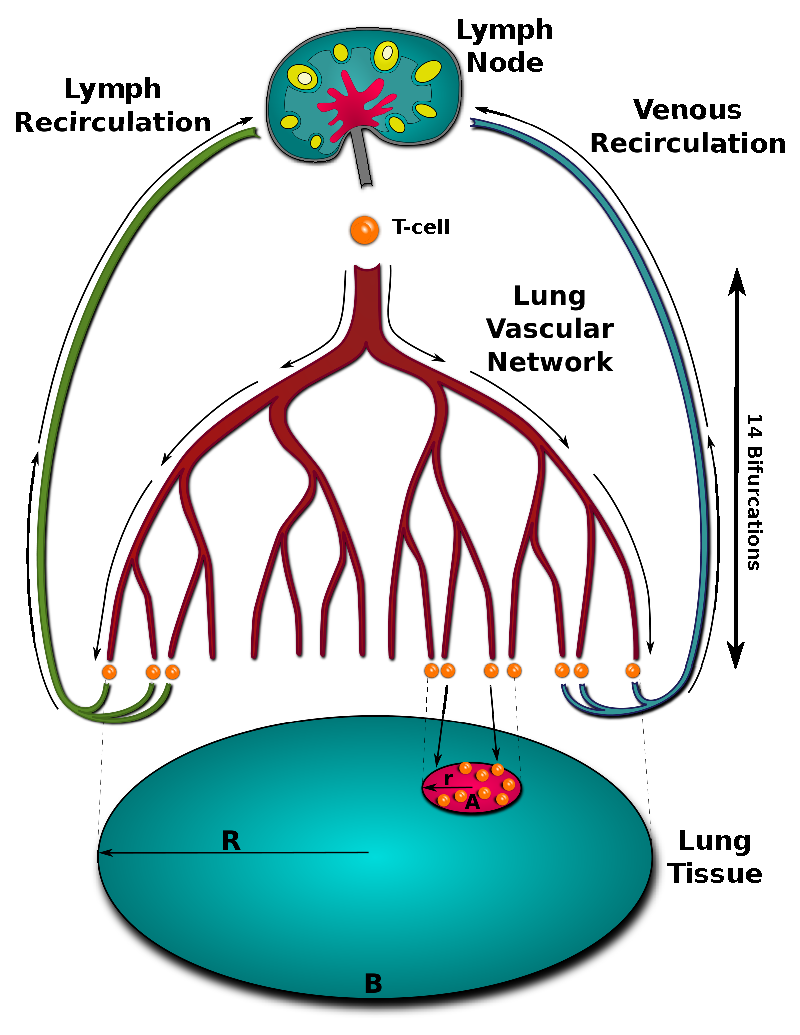
\includegraphics[width=4in]{Figure_1}
\end{center}
\caption{{\bf Model of T cell search.}  Activated T cells originate in the lymph node and enter the bloodstream after which they randomly navigate through 14 vascular bifurcations of the bronchial network.  Upon reaching a capillary, T cells exit into tissue if cytokine signal is present.  In the absence of signal, the T cell recirculates either through the lymph network or through the pulmonary vein back to the top of the network.}
\label{fig:systemchart}
\end{figure}

\begin{figure}[!ht]
\begin{center}
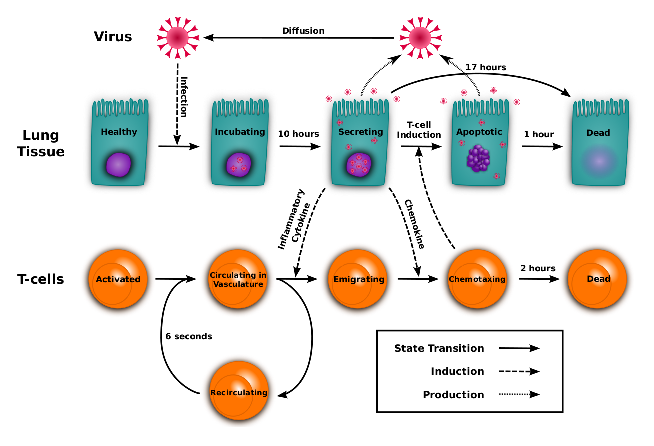
\includegraphics[width=4in]{Figure_2}
\end{center}
\caption{{\bf Visual representation of the model.}  Healthy epithelial cells infected by virus begin secreting virus after the incubation delay.  Activated T cells traverse the bronchial vascular network and may be recruited by inflammatory cytokine.  Chemotaxing T cells climb the chemokine gradient and induce apoptosis in infected cells.  Solid arrows represent a cell state transition from one behavior to another.  Dashed arrows display the mechanism used to induce a transition.  Dotted arrows indicate the production of new virus.}
\label{fig:modelchart}
\end{figure}

\begin{figure}[!ht]
\begin{center}
 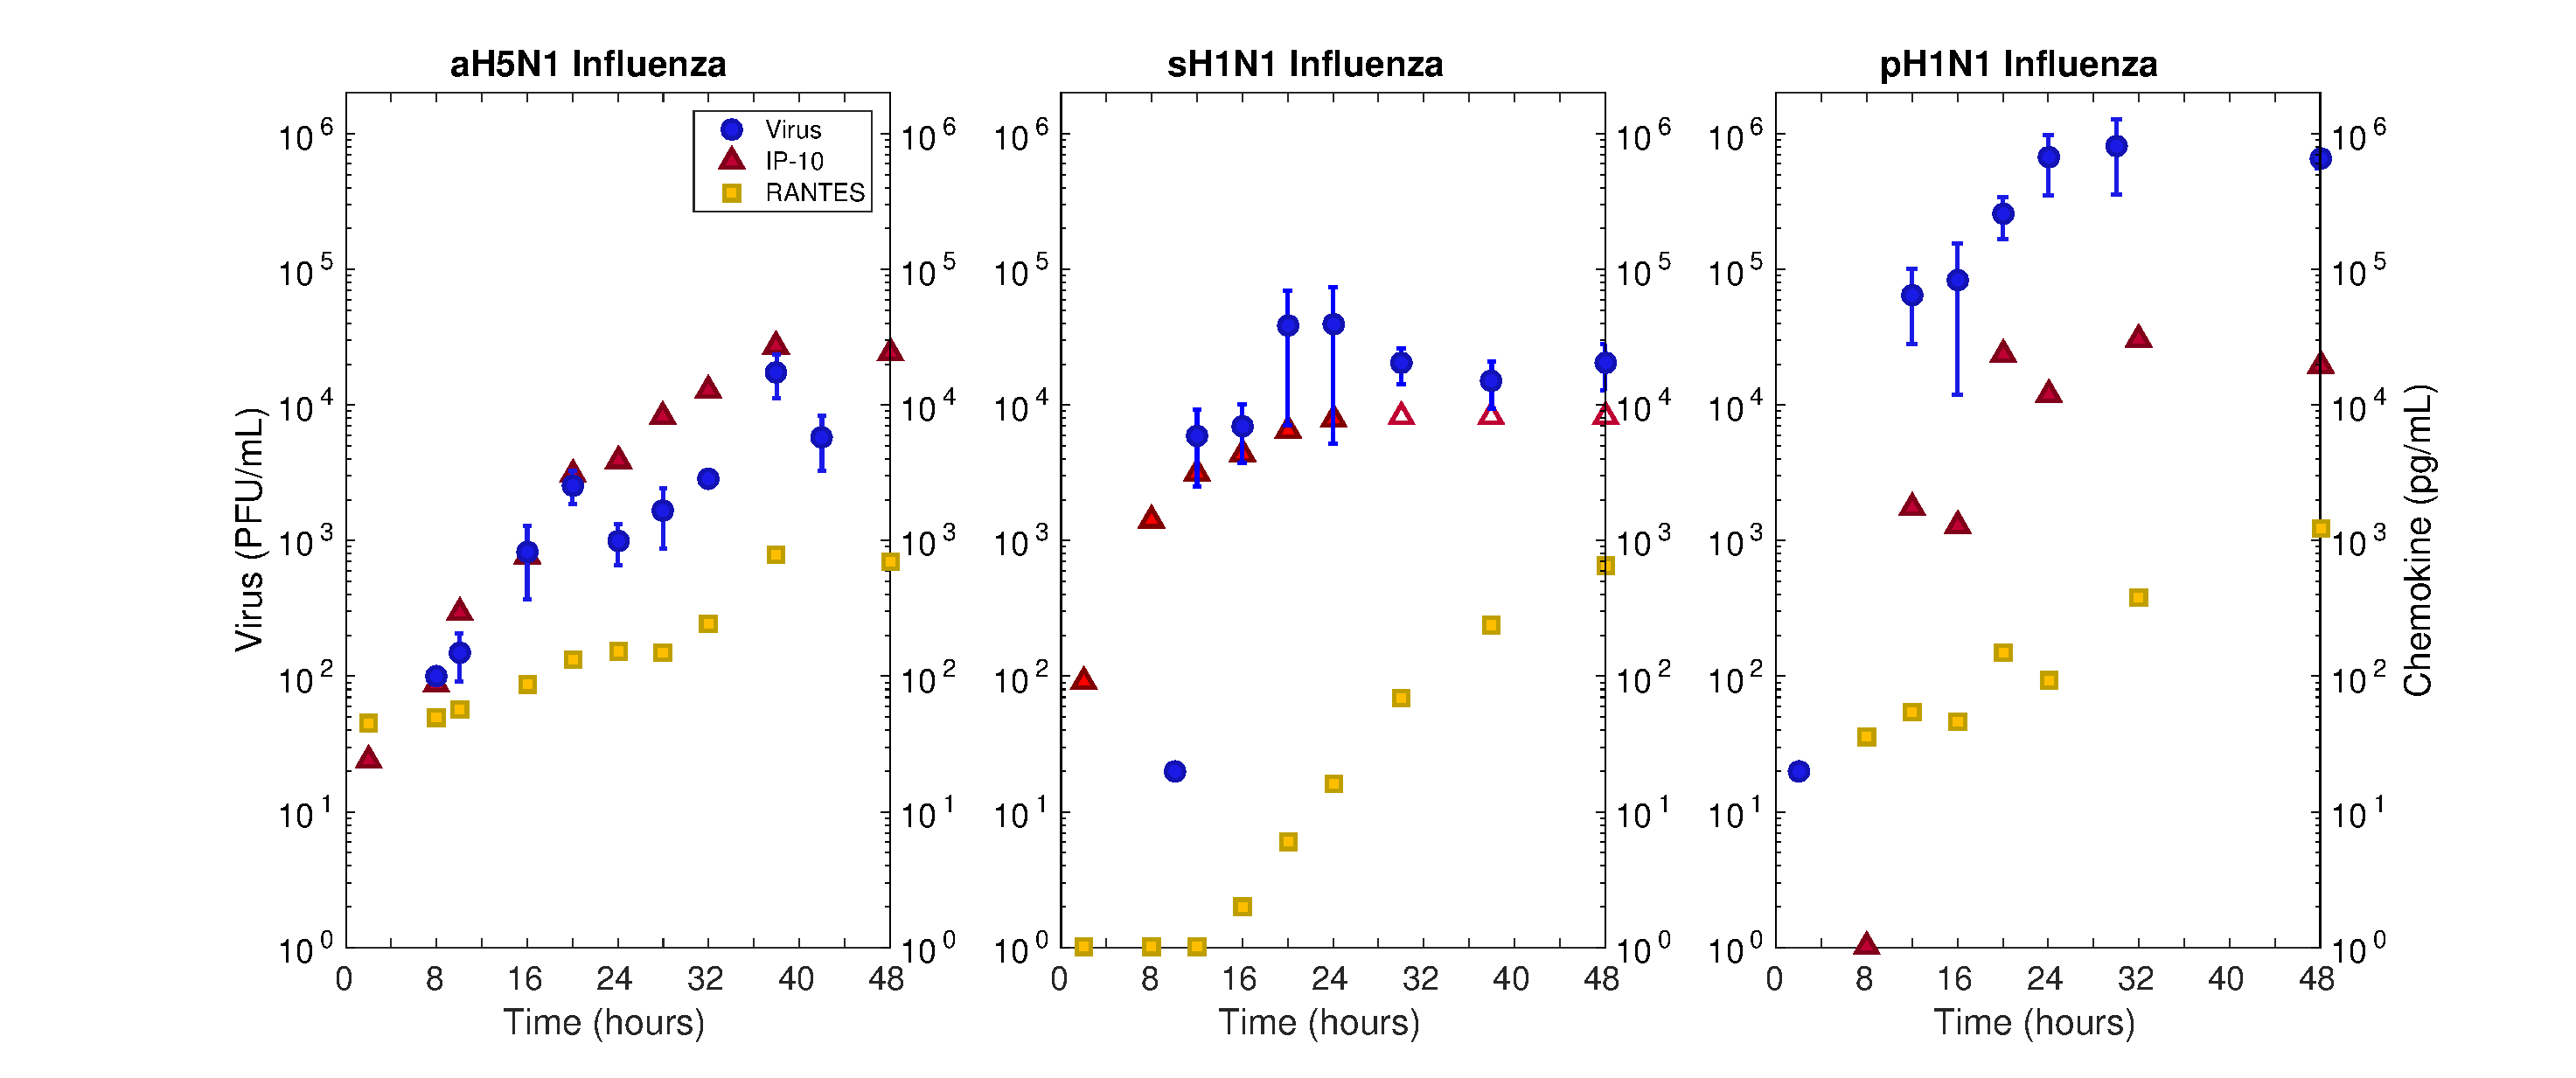
\includegraphics[width=\textwidth]{Figure_3}
 \end{center}
\caption{{\bf Empirical viral and cytokine titers for three strains of influenza: Avian H5N1, Seasonal sH1N1, and Pandemic pH1N1.}  Viral titer (blue circles) is in PFU/mL, and IP-10 (red triangle) and RANTES (yellow square) are shown in pg/mL.   sH1N1 IP-10 secretion exceeded measurement accuracy above 8500 pg/mL and these three values (empty red triangles) were not included in the model fitting.  An extended differential equation model from \citep{Mitchell2011} was fit to IP-10 and RANTES data (Equation 1) .  These fits were used to obtain chemokine production values for use in the spatial CyCells model.  Human bronchial epithelial cells were infected at an MOI of 0.01 (10,000 virions) with one of the three strains of influenza.  Apical fluid for viral secretion and basal media for chemokine secretion was collected at the given time intervals post infection.  Viral culture was performed by a standard plaque assay and chemokine levels were measured using 30 $\mu$l aliots for a panel of 17 chemokines and cytokines (not shown).} 
 \label{fig:data}
\end{figure}

\begin{figure}[ht!]
\begin{center}
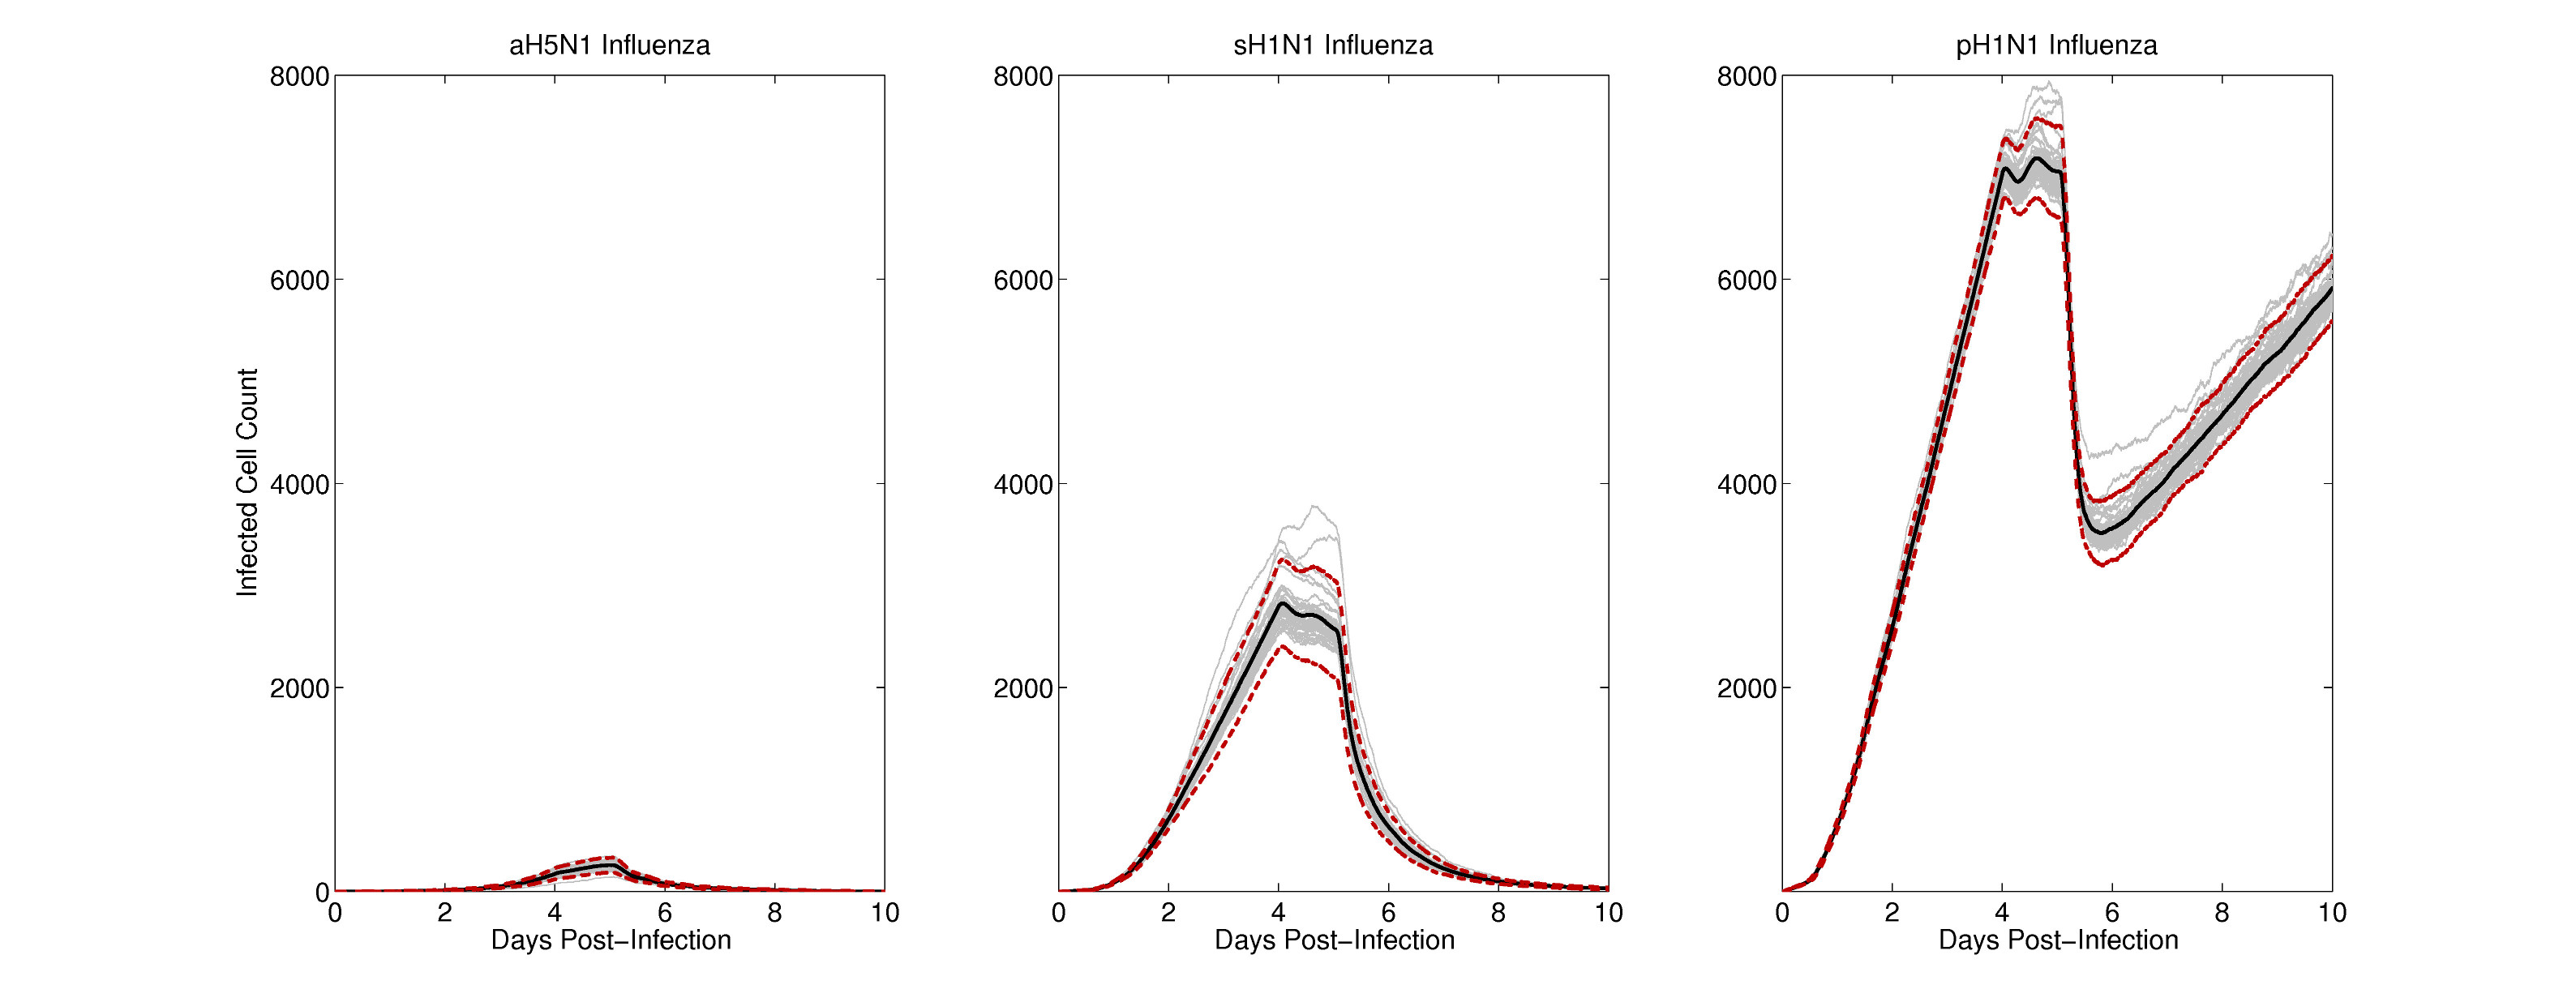
\includegraphics[width=\textwidth]{Figure_4}
 \end{center}
\caption{\textbf{Model results:} Time series plots of fifty runs of aH5N1 (A), sH1N1 (B), and pH1N1 (C) infections (gray). Each run took the calculated viral production and chemokine production rates for the three different strains of influenza as input (Table \ref{tab:strains}) and reported the total number of infected cells, including incubating, virus secreting and apoptotic, but not including dead cells.  Therefore the figures approximate the rate of plaque growth over time.  IP-10 and RANTES were simulated in each run, except for aH5N1, which  produced only RANTES.  Each run was initialized identically for each strain save for the random seed.  The middle line shows the mean while the red dashed lines show the 96\% credible confidence interval.} 
 \label{fig:variance}
\end{figure}

\begin{figure}[!ht]
\begin{center}
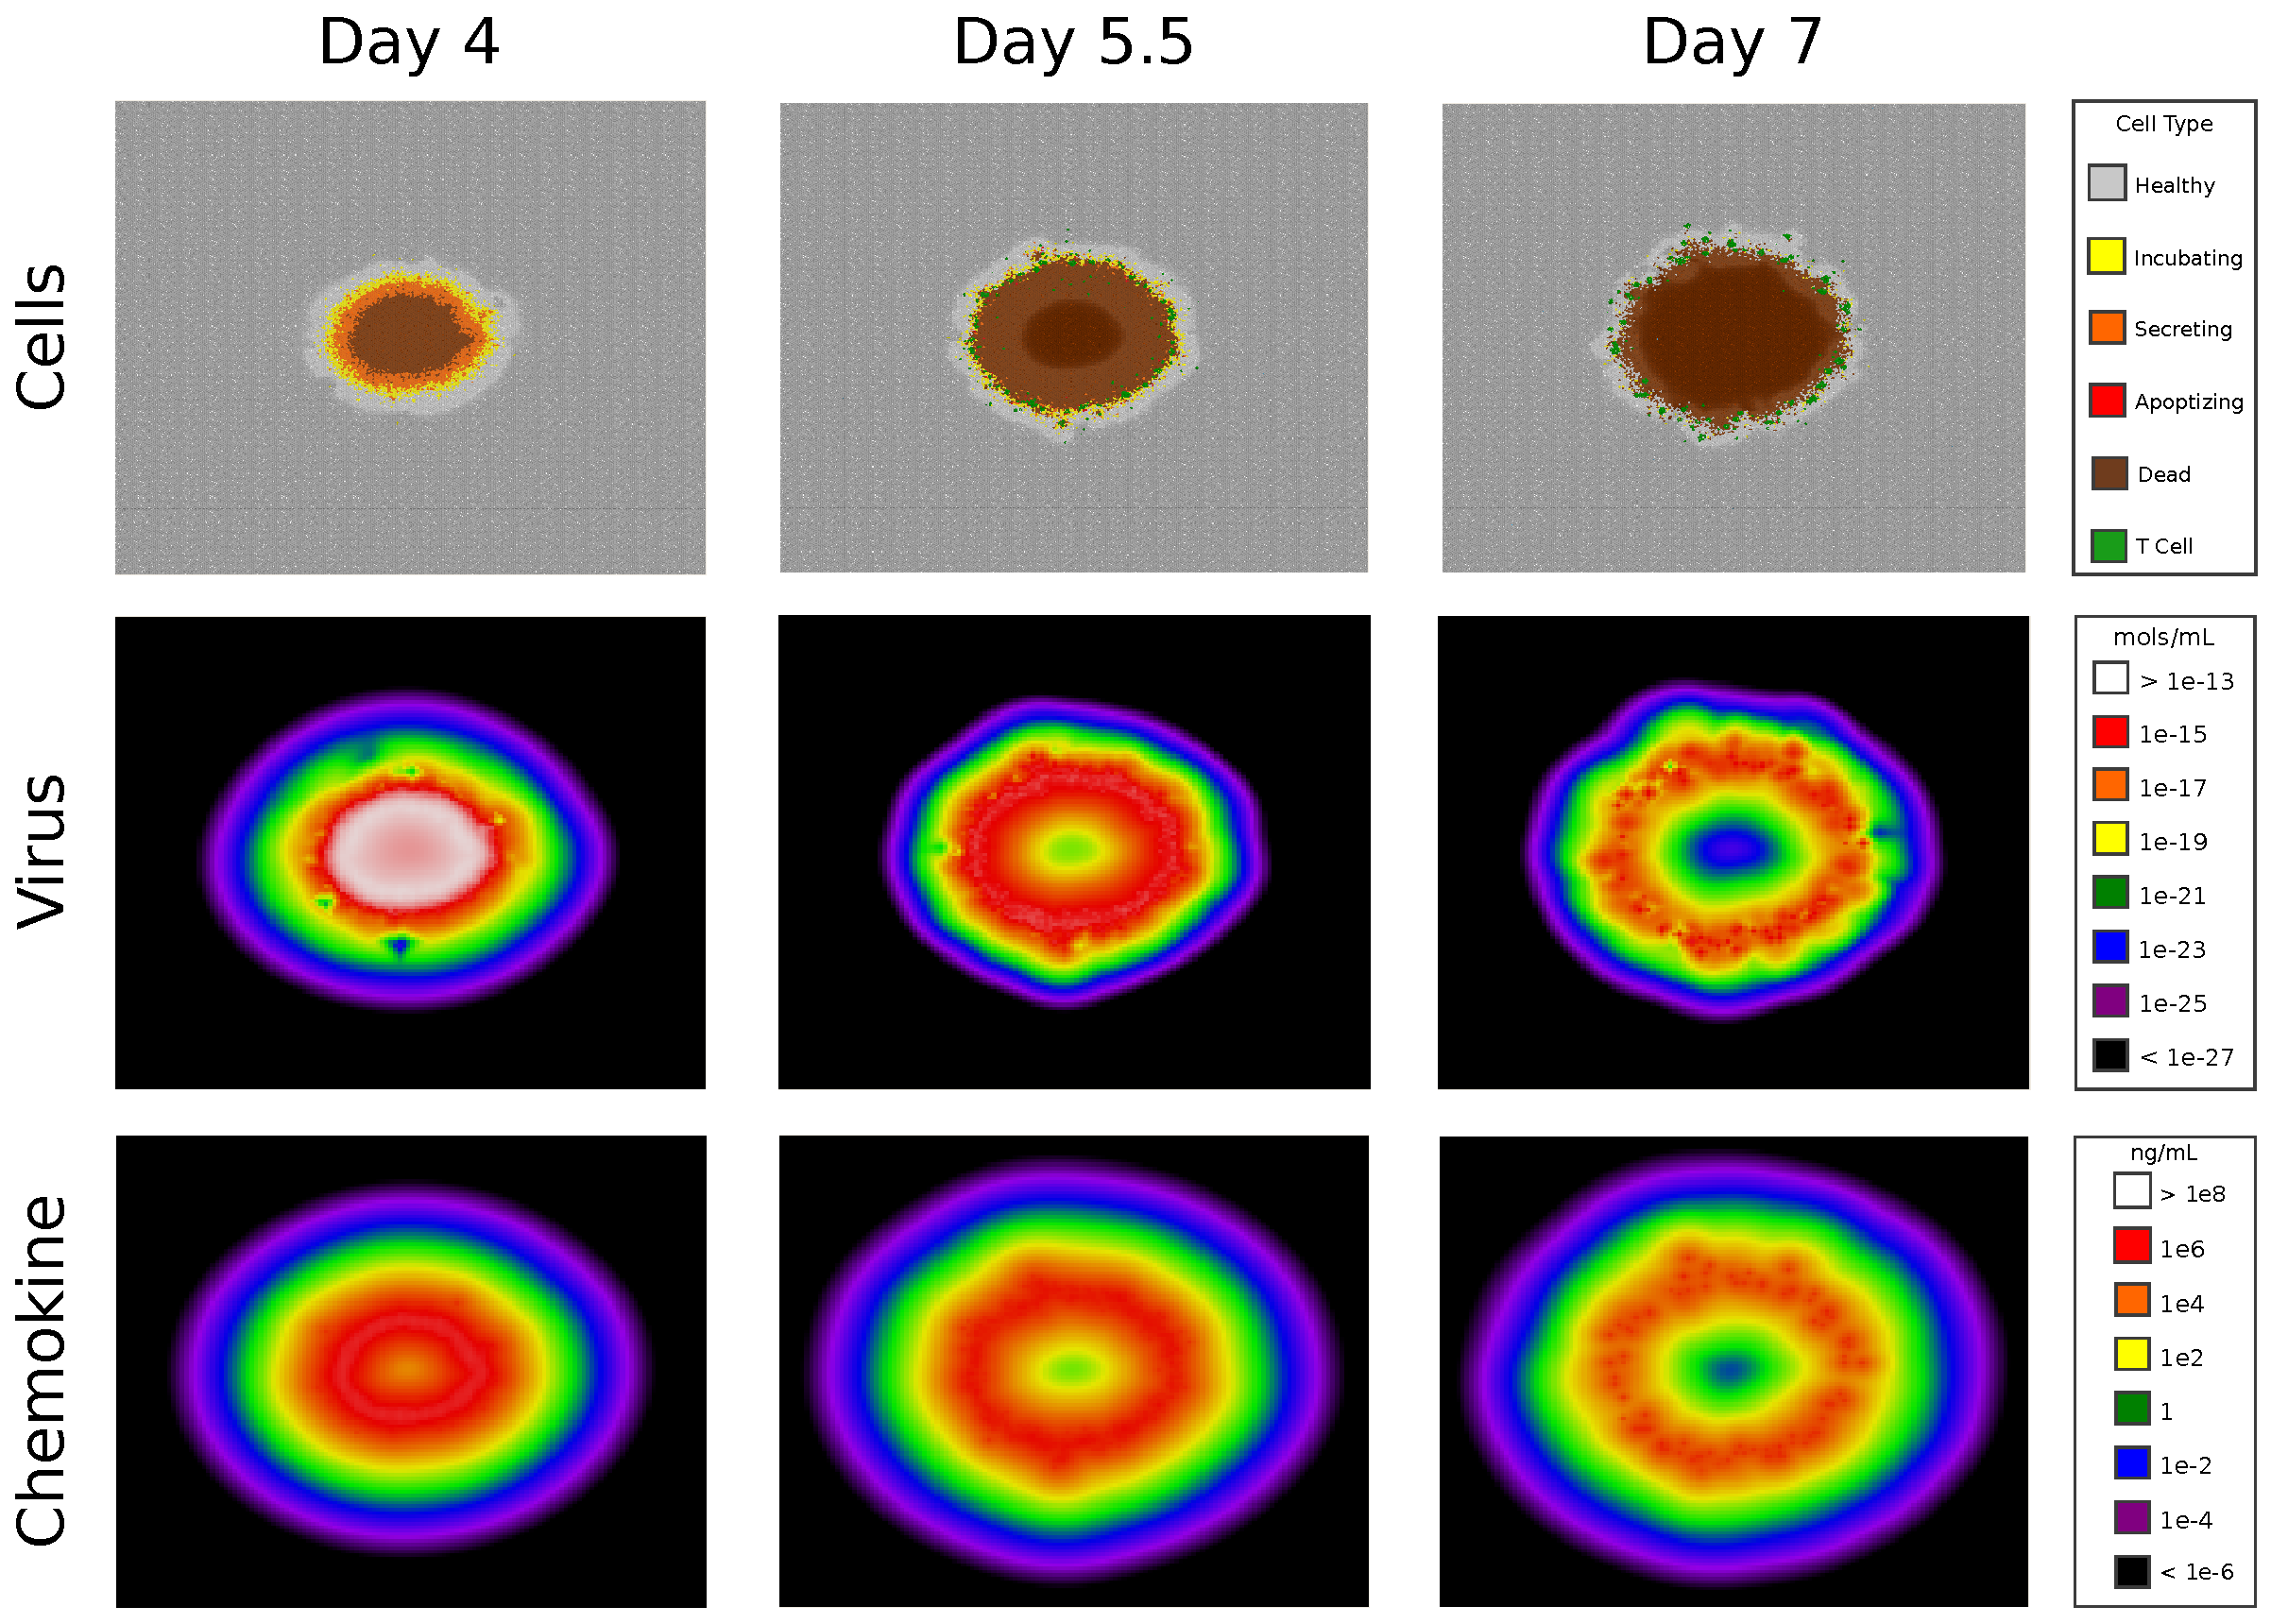
\includegraphics[width=\textwidth]{Figure_5}
 \end{center}
\caption{{\bf Simulated sH1N1 infection.} Screenshots from day 4, day 5.5, and day 7.  The top row shows the spreading focus of infection  through the color coding of individual cells:  healthy cells in uninfected tissue (gray),  virus-incubating cells (yellow), virus-secreting cells (orange), apoptotic cells (red), dead cells (brown), and T cells arriving at day 5 (green).  Free virus and chemokine particles are represented by compartmentalized concentrations of mols/mL and ng/mL.  Chemokine shown is an aggregate of total IP-10 and RANTES concentrations.  See Videos S1-S3 for an animated visualization of each row.} 
 \label{fig:cycells}
\end{figure}


\begin{figure}[!ht]
\begin{center}
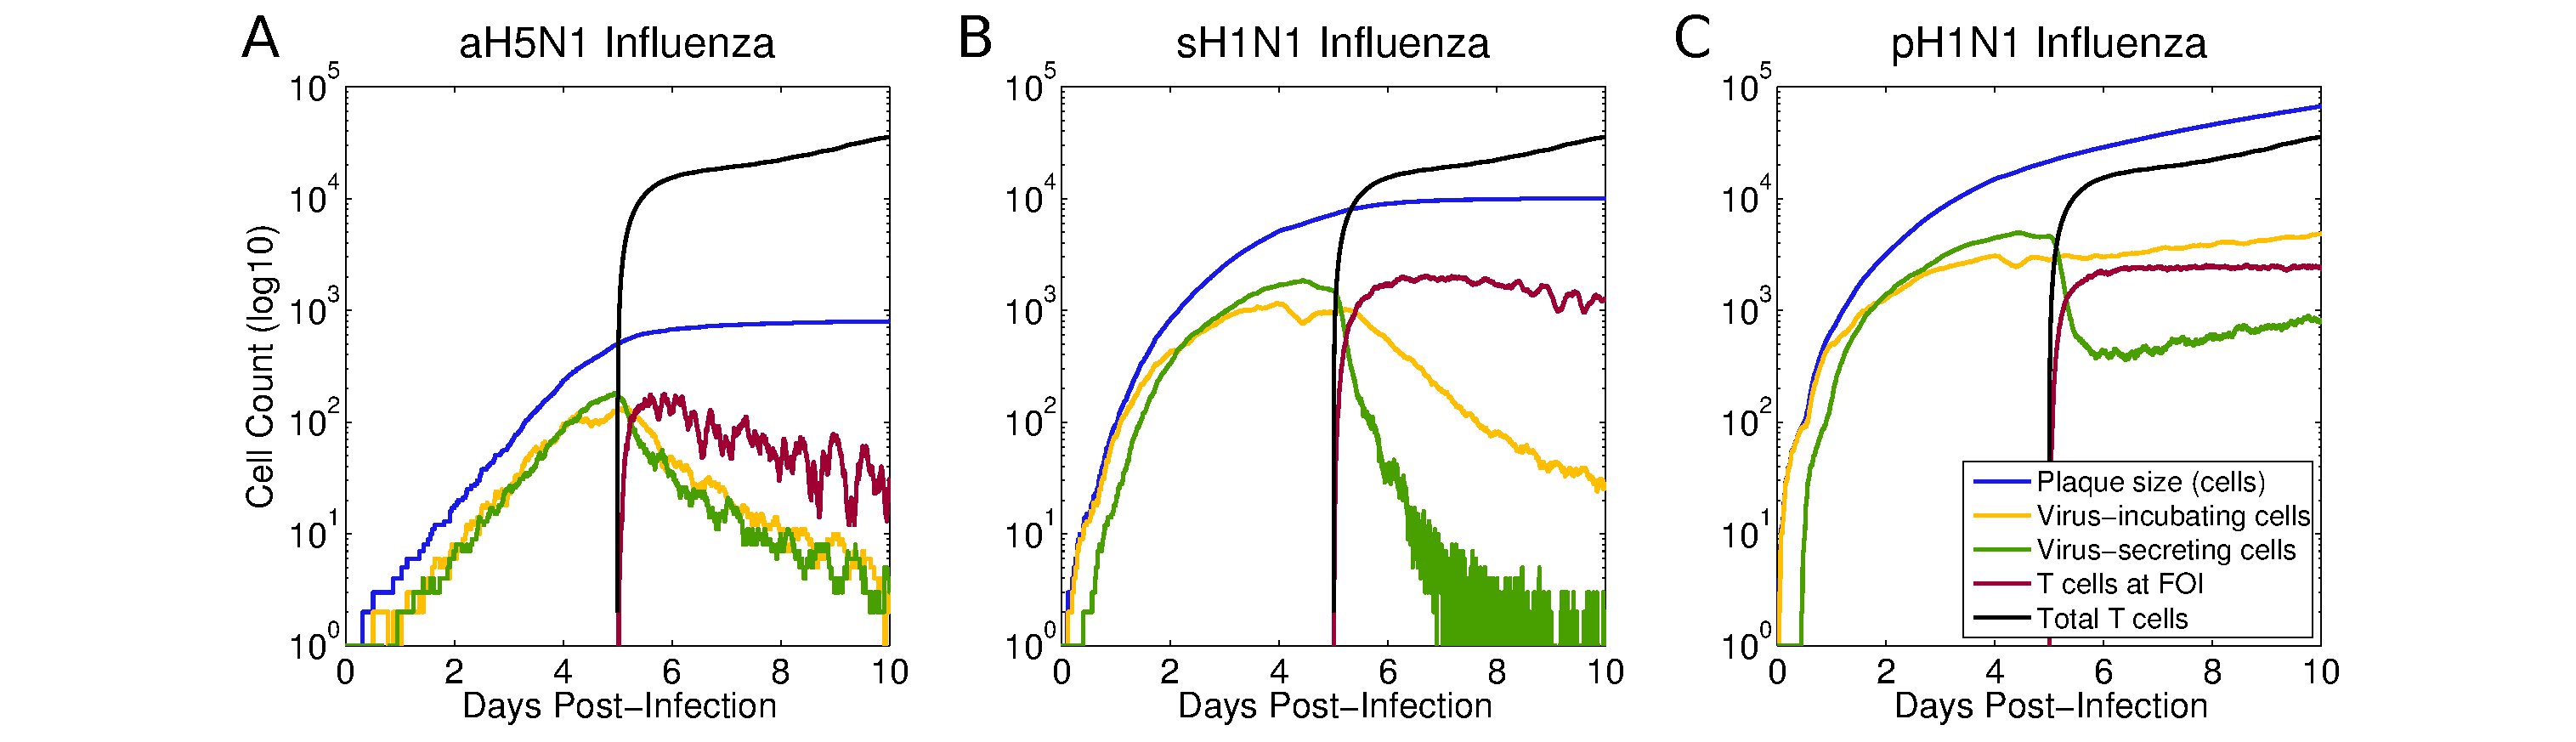
\includegraphics[width=\textwidth]{Figure_6}
 \end{center}
\caption{{\bf Simulated infections of aH5N1, sH1N1, and pH1N1.} Plotted values: total plaque size (blue), number of virus incubating cells (yellow), number of virus secreting cells (green), total number of T cells (black), and T cells at the focus of infection (FOI) (red).  T cells clear secreting and incubating cells in aH5N1, fail to clear incubating cells in sH1N1, and fail to clear either type of infected cell in pH1N1.  The number of incubating cells (yellow) after day 5 differs markedly among the three strains indicating that the T cells have differing success at controlling the infection.} 
 \label{fig:plaquesize}
\end{figure}


\begin{figure}[!ht]
\begin{center}
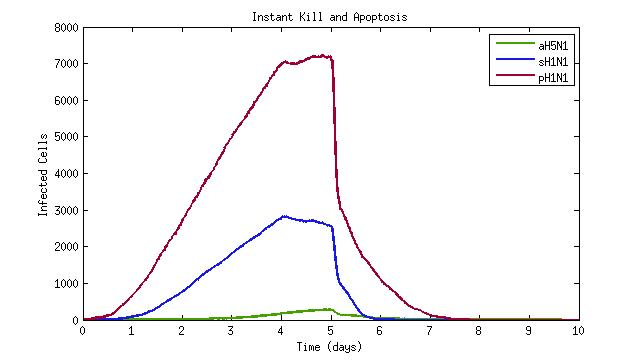
\includegraphics[width=4in]{Figure_7}
 \end{center}
\caption{{\bf Simulated infections of aH5N1, sH1N1, and pH1N1 with instant cell death.} The model results how that the combined delay of the T cell kill time and apoptosis time form a barrier to infection clearance.  Removing both delays results in infection clearance for all strains.}
 \label{fig:instantkill}
\end{figure}

%\setcounter{figure}{0}
%\renewcommand{\thefigure}{S\arabic{figure}}
%
%\begin{figure}[ht!]
%\begin{center}
%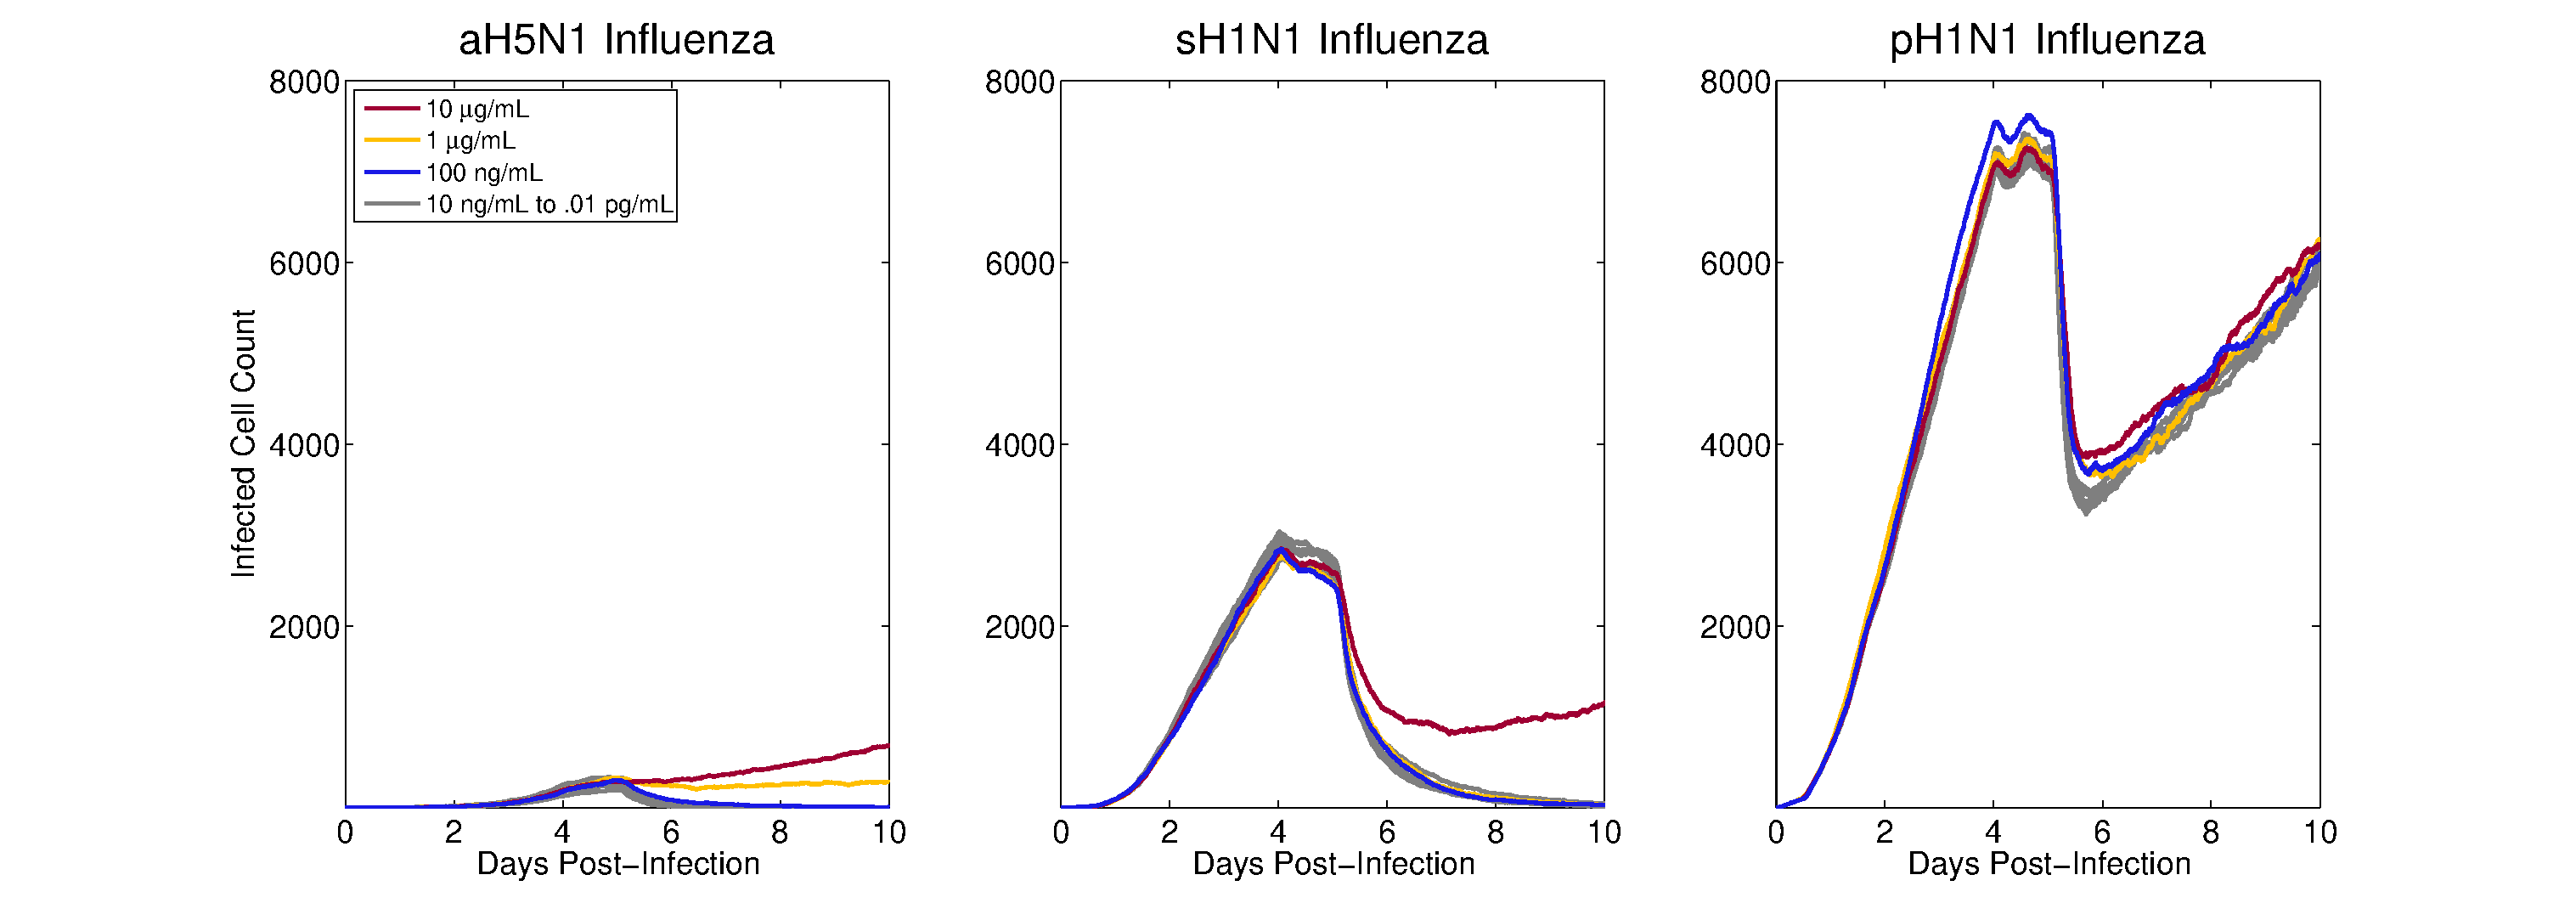
\includegraphics[width=\textwidth]{Figure_S1}
% \end{center}
%\caption{{\bf Varying T cell sensitivity to chemokine.}  H5N1 model results use RANTES  only, and sH1N1 and pH1N1 use both IP-10 and RANTES. Total number of incubating, secreting and apoptotic cells are plotted for each infection.  The sensitivity value specifies the minimum level of chemokine concentration required for T cells to detect it.} 
%\end{figure}
%
%
%\begin{figure}[!ht]
%\begin{center}
%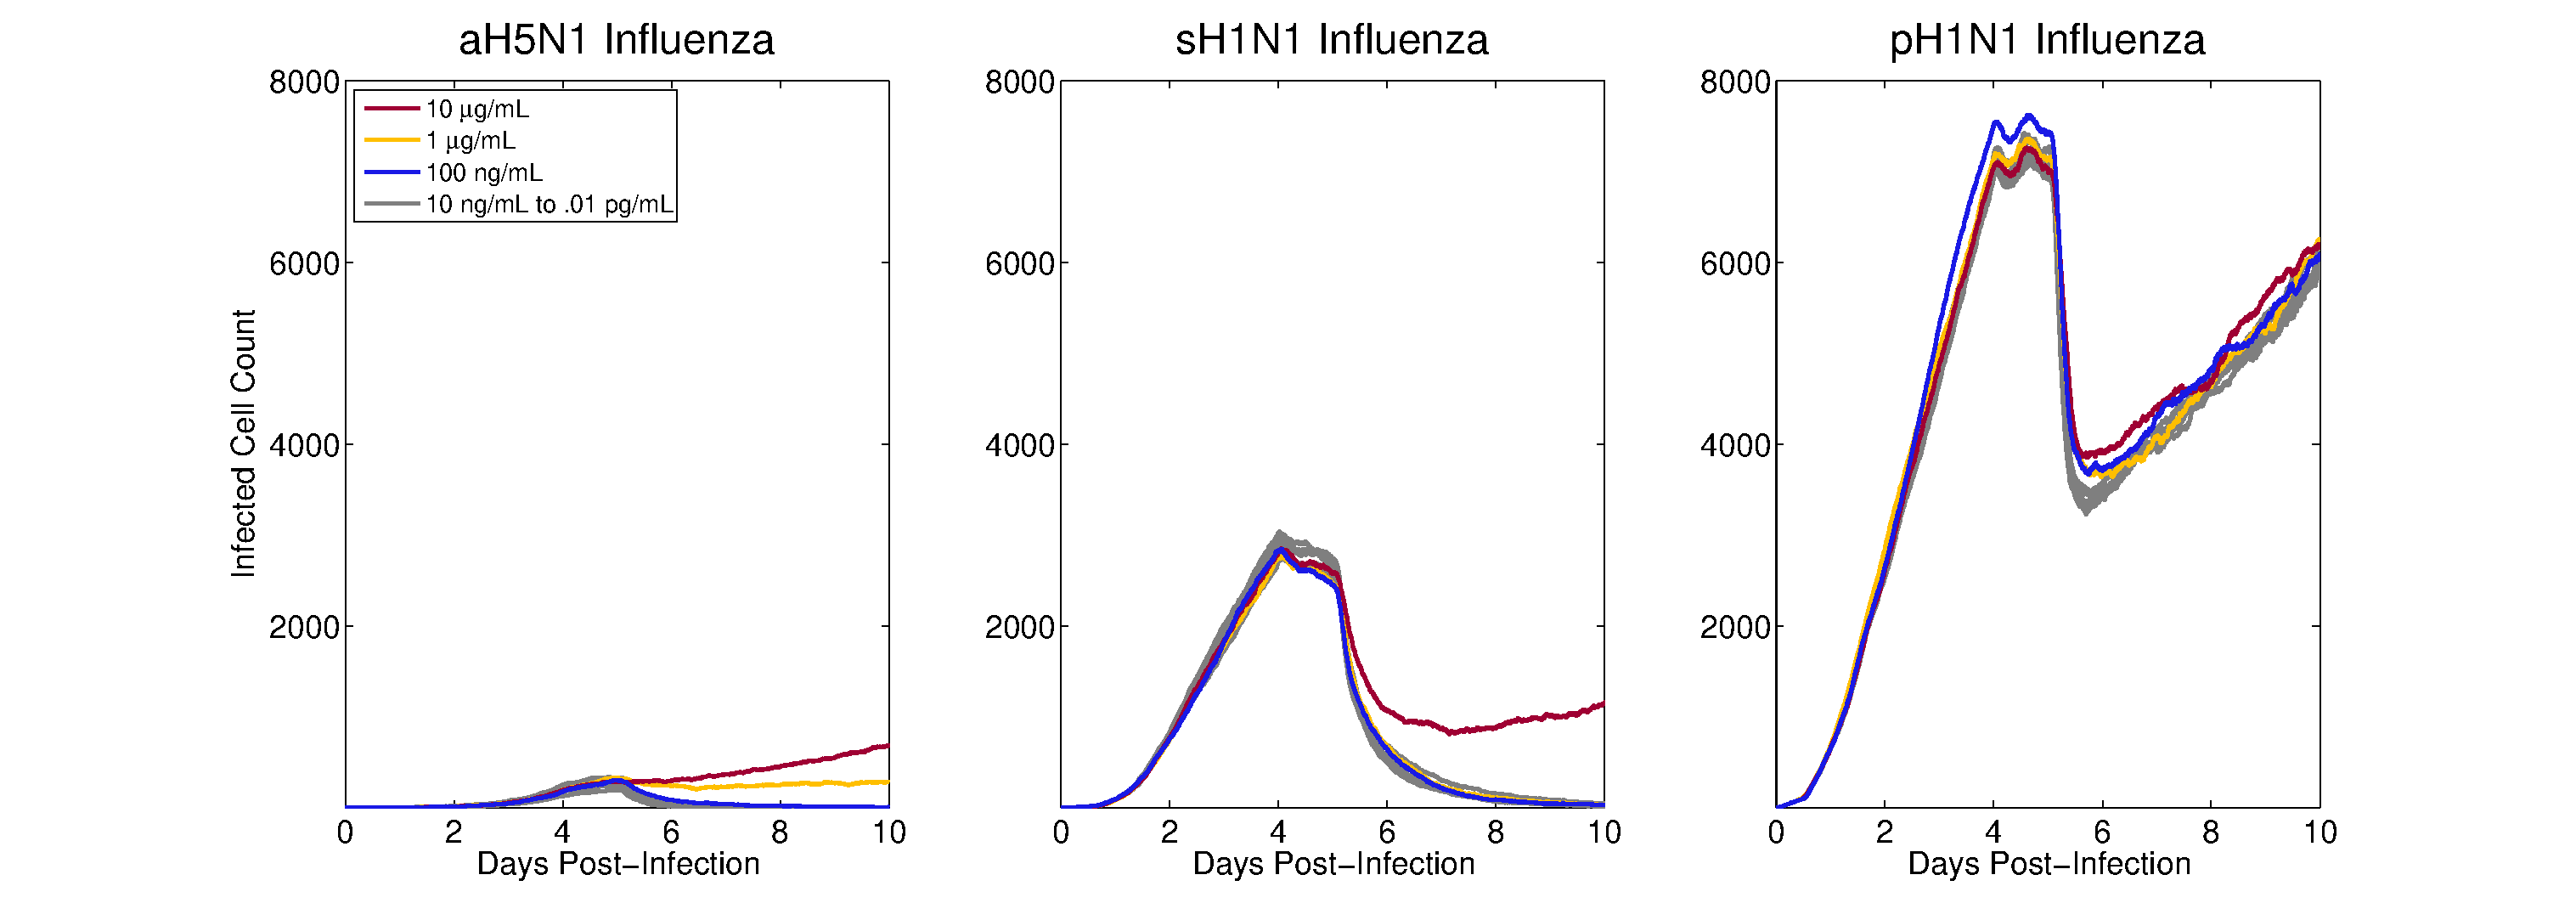
\includegraphics[width=4in]{Figure_S2}
% \end{center}
%\caption{\textbf{Effects of different chemokine combinations.}  A) aH5N1 does not stimulate an IP-10 response.  B-C) sH1N1 and pH1N1 show no significant difference between IP-10 alone versus IP-10 and RANTES combined.} 
% \label{fig:sensitivity}
%\end{figure}
%
%\setcounter{figure}{0}
%\renewcommand{\figurename}{Video}
%
%\begin{figure}[ht!]
%\caption{The first of three overlaid videos of a representative seasonal H1N1 infection.  This video spans the 10 day infection and shows the cells as they transition from healthy to infected to dead.  T cells show half way through the simulation.  Healthy cells are gray, virus-incubating cells are yellow, virus-secreting cells are orange, apoptotic cells are red, and T cells are green.} 
% \label{video:cell_view}
%\end{figure}
%
%\begin{figure}[ht!]
%\caption{The second of three overlaid videos of a representative seasonal H1N1 infection.  This video spans the 10 day infection and shows the virus concentration.  Notice the volatility when T cells arrive halfway through the simulation.  Virus concentration ranges from 1e-13 mols/mL (white) to 1e-27 mols/mL (black).  Refer to Figure 5 for the detailed legend. } 
% \label{video:virus_view}
%\end{figure}
%
%\begin{figure}[ht!]
%\caption{The third of three overlaid videos of a representative seasonal H1N1 infection.  This video spans the 10 day infection and shows the chemokine concentration.  Notice the volatility when T cells arrive halfway through the simulation.  Chemokine concentration ranges from 1e8 ng/mL (white) to 1e-6 ng/mL (black).  Refer to Figure 5 for the detailed legend. } 
% \label{video:chemokine_view}
%\end{figure}
%
%\begin{figure}[ht!]
%\caption{A closer look at the 2009 pandemic simulation.  This video shows the infection from day 6 to day 7 with each frame spanning 60 simulated seconds.  Healthy cells are gray, virus-incubating cells are yellow, virus-secreting cells are orange, apoptotic cells are red, and T cells are green.  Note the high proportion of virus-secreting cells (orange) early on.  As time passes, secreting cells are gradually contained to the point where they become very sparse.  T cell clumping often prevents the T cells from quick discovery of new secreting cells.}
%\end{figure}

\pagebreak

\section*{Tables}
%\begin{table}[!ht]
%\caption{
%\bf{Table title}}
%\begin{tabular}{|c|c|c|}
%table information
%\end{tabular}
%\begin{flushleft}Table caption
%\end{flushleft}
%\label{tab:label}
% \end{table}



\begin{table}[!ht]
\centering
\begin{tabular}{ | r | c | c | c | }
  \hline                        
  \multicolumn{1}{|c|}{\multirow{2}{*}{Strain}} & IP-10 Production & RANTES Production & Viral Production \\
   & \footnotesize{$(pg/s\cdot cell)$}  & \footnotesize{$(pg/s\cdot cell)$} &  \footnotesize{$(PFU/s\cdot cell)$} \\
  \hline
  \multirow{2}{*}{Avian H5N1} & 2.0e-4 &  1.3e-5 & 5.4e-5 \\
   &  \footnotesize{8.4e-5 --- 4.2e-4} & \footnotesize{7.9e-6 --- 1.9e-5} & \footnotesize{4.4e-5 --- 3.7e-4}\\ 
   \hline
  \multirow{2}{*}{Seasonal H1N1} & 1.8e-4 &  8.9e-7 & 3.8e-4 \\
   & \footnotesize{1.2e-4 --- 3.0e-4} & \footnotesize{4.8e-7 --- 1.6e-6} & \footnotesize{2.8e-4 --- 1.5e-3}\\
   \hline
  \multirow{2}{*}{Pandemic H1N1} & 8.7e-5 &  4.3e-6 & 5.1e-3 \\
   & \footnotesize{1.7e-5 --- 7.1e-4} & \footnotesize{5.0e-7 --- 3.5e-5} & \footnotesize{2.8e-3 --- 5.3e-3} \\
  \hline
\end{tabular}
\caption{Strain-specific parameters.  Small text values show 95\% confidence intervals resulting from 1,000 bootstrapping runs for each parameter \citep{Wu1986}.  Bootstrapping for the chemokine values was performed using the original fit of Eq. S1 to the data in Fig.~\ref{fig:data} to produce new data sets.  Viral production values and confidence intervals are taken from \citep{Mitchell2011}.}
\label{tab:strains}
\end{table}

\begin{table}[!ht]
\begin{center}
\begin{tabular}{| l | c | l l l | c |}
  \hline                        
  Referenced Parameters & Units & Min & Value & Max & Source \\
  \hline
  $^{\dagger}$Viral Diffusion in Airway & \textit{$\mu$m$^2$/s} & 3.18e-4 & \textbf{3.18e-2} & 3.18  & \citep{Beauchemin2006} \\
  $^{\dagger}$Viral Decay in Airway & \textit{day$^{-1}$} & 0.01 & \textbf{1} & 100 & \citep{Lee2009} \\
  Chemokine Diffusion Rate & \textit{$\mu$m$^2$/s} & 3.18e-3 & \textbf{.318} & 318 & \citep{Beauchemin2006} \\
  Incubation Time & \textit{hours} & 5 & \textbf{10} & 20 & \citep{Mitchell2011} \\
  Epithelial Cell Radius & \textit{$\mu$m} & | & \textbf{5} & | & \citep{Elbert1999} \\
  T Cell Radius & \textit{$\mu$m} & | & \textbf{5} & | & \citep{abbas2011cellular} \\
  T Cell Production Rate & \textit{cells/h} & 125 & \textbf{1,257} & 3,750 & \citep{Miao2010a} \\ 
  T Cell Speed & \textit{$\mu$m/min} & 6e-2 & \textbf{6} & 600 & \citep{Egen2011} \\
  Blood Circulation Time & \textit{seconds} & 1 & \textbf{6} & 3,600 & \citep{Banerjee2010b} \\
  T Cell Sensitivity to Chemokine & \textit{ng/mL} & | & \textbf{100} & | & \citep{Nandagopal2011} \\
  Onset of T Cell Lymph Node Exit & \textit{days }& | & \textbf{5} & | & \citep{Banerjee2011} \\
  $^{\dagger}$IgM Viral Decay Factor & | & 1 & \textbf{10} & 1,000 & \citep{Diamond2003} \\
  IgM Onset & \textit{days} & | & \textbf{4} & | & \citep{Diamond2003} \\
  \hline
  \hline                        
  Estimated Parameters$^*$ & Units & Min & Value & Max & Footnote \\
  \hline
  Chemokine Decay Rate & \textit{Hz} & 3.8e-6 & \textbf{3.8e-4} & 3.8e-2 & 1\\
  $^{\dagger}$Infectivity & \textit{min/virion} & 12 & \textbf{120} & 1,200   &  2 \\
  Expression Time & \textit{min} & 100 & \textbf{1,000} & 3,000 & \citep{Mitchell2011}$^3$ \\
  T Cell Expected Kill Time & \textit{min} & 0 & \textbf{10} & 100 & 4 \\
  Apoptosis Time & \textit{hours} & 0 & \textbf{1} & 2 & \citep{Ganusov2008}$^5$ \\
  T Cell Age (at FOI) & \textit{min} & 12 & \textbf{120} & 1,200 & 6 \\
  T Cell Age (in Blood) & \textit{days} & 0.04 & \textbf{4} & 400 & 6 \\
  \hline  
\end{tabular}
\caption{Default values used for the model in bold.  Min and max represent the extreme values tested in the sensitivity analysis (Table~\ref{tab:sensitivity} and Fig.~S3-5).  $^*$ All estimated parameter values are examined in the sensitivity analysis (Table~\ref{tab:sensitivity}, S2.3).  $^{\dagger}$ denotes parameters determined to be sensitive by the one-factor-at-a-time sensitivity analysis.  Values were taken from experimental literature if possible and from earlier modeling papers if not.  Parameters not found in literature were estimated as follows.  1) Corresponds to a 30 minute half-life.  2) Epithelial cells are infected at a probabilistic rate such that the expected time for infection in the presence of a single virion is 2 hours.  This scales linearly with the number of virions in the cell's vicinity.  3) Chosen as a plausible median time (1,000 minutes) between 6 hours and 24 hours.  4) T cells induce apoptosis in nearby virus-secreting epithelial cells at a probabilistic rate such that the expected time to induce apoptosis is 10 minutes.  This rate does not scale with T cell numbers.  5) Calculated for low T cell densities.  6) Chosen to be at the lower end of biologically plausible values because increased T cell counts are shown not to affect the model behavior. }
\label{tab:parameters}
\end{center}
\end{table}
% 7) IgM presence is abstracted by increasing viral decay by a factor of ten. $^\ddagger$Activated T Cell.  $^\ast$Focus of Infection.


\begin{table}[!ht]
\begin{center}
\begin{tabular}{| c | l | c c c |}
  \hline                        
  Category & Parameter & Avian H5N1 & Seasonal H1N1 & Pandemic H1N1 \\
  \hline
  \multirow{3}{*}{Chemokine} & Chemokine Decay Rate & \cellcolor{blue!30}bounded stable & \cellcolor{blue!30}bounded stable & \cellcolor{green!50}stable \\
  & Chemokine Diffusion Rate & \cellcolor{blue!30}bounded stable & \cellcolor{green!50}stable& \cellcolor{green!50}stable \\
  & Chemokine Secretion Rate & \cellcolor{blue!30}bounded stable & \cellcolor{green!50}stable & \cellcolor{green!50}stable \\
  \hline
  \multirow{6}{*}{T Cell} & Circulation Time & \cellcolor{blue!30}bounded stable & \cellcolor{blue!30}bounded stable & \cellcolor{blue!30}bounded stable \\
  & T Cell Kill Rate & \cellcolor{green!50}stable & \cellcolor{blue!30}bounded stable & \cellcolor{blue!30}bounded stable \\
  & T Cell Speed & \cellcolor{green!50}stable & \cellcolor{blue!30}bounded stable & \cellcolor{blue!30}bounded stable \\
  & T Cell Age in Blood & \cellcolor{green!50}stable & \cellcolor{blue!30}bounded stable& \cellcolor{blue!30}bounded stable \\
  & T Cell Age at FOI & \cellcolor{green!50}stable & \cellcolor{blue!30}\textbf{bounded stable$^\dagger$} & \cellcolor{blue!30}bounded stable \\
  & T Cell Production Rate & \cellcolor{blue!30}bounded stable & \cellcolor{blue!30}bounded stable & \cellcolor{blue!30}bounded stable \\
  \hline
  \multirow{3}{*}{Delay} & Apoptosis Time & \cellcolor{green!50}stable & \cellcolor{green!50}stable & \cellcolor{green!50}stable \\
  & Expression Time & \cellcolor{yellow!50}peak change & \cellcolor{yellow!50}\textbf{peak change$^\dagger$} & \cellcolor{yellow!50}peak change \\
  & Incubation Time &  \cellcolor{yellow!50}peak change & \cellcolor{yellow!50}peak change & \cellcolor{yellow!50}peak change \\
  \hline 
  \multirow{4}{*}{Virus} & Viral Response to IgM & \cellcolor{red!40}sensitive & \cellcolor{red!40}\textbf{sensitive$^\dagger$} & \cellcolor{red!40}sensitive \\
  & Infectivity & \cellcolor{red!40}sensitive & \cellcolor{red!40}\textbf{sensitive$^*$} & \cellcolor{red!40}sensitive \\
  & Viral Decay Rate & \cellcolor{red!40}sensitive & \cellcolor{red!40}\textbf{sensitive$^*$} & \cellcolor{red!40}sensitive \\
  & Viral Diffusion Rate & \cellcolor{red!40}sensitive & \cellcolor{red!40}\textbf{sensitive$^*$} & \cellcolor{red!40}sensitive \\
  \hline  
\end{tabular}
\caption{\textbf{Sensitivity Results:} The above parameters were varied over predetermined ranges in isolation, resulting in new model runs for every new value tested (Figs. S3-S5).  The results of the sensitivity analysis were then qualitatively evaluated for each individual parameter.  A model run's behavior was determined by examining the height of the peak of the infection at day 5 post-infection and the number of infected cells at day 10 post-infection.  Each combination of influenza strain and free parameter was classified as belonging to one of four categories.  Parameters were classified as \textbf{stable} if all runs follow the same behavior, \textbf{bounded stable} if intermediate parameter adjustments did not affect the model's behavior, even if the more extreme adjustments did, \textbf{peak change} if the peak of the infection differs but the result at day 10 is the same, and \textbf{sensitive} if any level of change in the parameter affects the resulting model behavior.  PRCC analysis was also performed for the sH1N1 strain over these parameters (Figs. S6-S8).  Bold text in the seasonal column denotes significant Spearman rank correlation ($p < 0.01$) over the time period where the parameter was active. $\dagger$ indicates a maximum \textit{absolute} Spearman's $\rho$ of less than 0.5.  $*$ indicates a maximum \textit{absolute} Spearman's $\rho$ of over 0.5.}
\label{tab:sensitivity}
\end{center}
\end{table}
% 7) IgM presence is abstracted by increasing viral decay by a factor of ten. $^\ddagger$Activated T Cell.  $^\ast$Focus of Infection.



\end{document}

